
\documentclass[reqno,12pt,oneside]{report} % right-side equation numbering, 12 point font, print one-sided 
%\documentclass[reqno,12pt,twoside,openright]{report} % right-side equation numbering, 12 point font, print two-sided, Chapters start on odd pages. 

\usepackage{rac}         % Use Rackham thesis style file
\usepackage{aas_macros}  % To allow the reading of ADS journal references in the bibliography
\usepackage[intlimits]{amsmath} % Puts the limits of integrals on top and bottom
\usepackage{amsxtra}     % Use various AMS packages
\usepackage{amsthm}
\usepackage{amssymb}
\usepackage{amsfonts}
\usepackage{graphicx}    % Add some packages for figures. Read epslatex.pdf on ctan.tug.org
\usepackage{rotating}
\usepackage{color}
\usepackage{epsfig}
\usepackage{subcaption}   % To make subfigures. Read subfigure.pdf on ctan.tug.org
\usepackage{verbatim}
\usepackage{natbib}      % Allows you to use BibTeX
\usepackage[printonlyused]{acronym} % For the List of Abbreviations. Read acronym.pdf on ctan.tug.org
\usepackage{setspace}    % Allows you to specify the line spacing
\captionsetup{compatibility=false}
\doublespacing           % \onehalfspacing for 1.5 spacing, \doublespacing for 2.0 spacing.
\newcommand{\sun}{\ensuremath{\odot}} % sun symbol is \sun
%%%%%%%%%%%%%%%%%%%%%%%%%%%%%%%%%%%%%%%%%%%%%%%%%%%%%%%%%%%%%%%%%%%%%%%%%%%%%%%

% Various theorem environments. All of the following have the same numbering
% system as theorem.

\theoremstyle{plain}
\newtheorem{theorem}{Theorem}
\newtheorem{prop}[theorem]{Proposition}
\newtheorem{corollary}[theorem]{Corollary}
\newtheorem{lemma}[theorem]{Lemma}
\newtheorem{question}[theorem]{Question}
\newtheorem{conjecture}[theorem]{Conjecture}
\newtheorem{assumption}[theorem]{Assumption}

\theoremstyle{definition}
\newtheorem{definition}[theorem]{Definition}
\newtheorem{notation}[theorem]{Notation}
\newtheorem{condition}[theorem]{Condition}
\newtheorem{example}[theorem]{Example}
\newtheorem{introduction}[theorem]{Introduction}

\theoremstyle{remark}
\newtheorem{remark}[theorem]{Remark}
%%%%%%%%%%%%%%%%%%%%%%%%%%%%%%%%%%%%%%%%%%%%%%%%%%%%%%%%%%%%%%%%%%%%%%%%%%%%%%%

\numberwithin{theorem}{chapter}     % Numbers theorems "x.y" where x
                                    % is the section number, y is the
                                    % theorem number

%\renewcommand{\thetheorem}{\arabic{chapter}.\arabic{theorem}}

%\makeatletter                      % This sequence of commands will
%\let\c@equation\c@theorem          % incorporate equation numbering
%\makeatother                       % into the theorem numbering scheme

%\renewcommand{\theenumi}{(\roman{enumi})}

%%%%%%%%%%%%%%%%%%%%%%%%%%%%%%%%%%%%%%%%%%%%%%%%%%%%%%%%%%%%%%%%%%%%%%%%%%%%%%

% If printing two-sided, this makes sure that any blank page at the 
% end of a chapter will not have a page number. 
\makeatletter
\def\cleardoublepage{\clearpage\if@twoside \ifodd\c@page\else
\hbox{}
\thispagestyle{empty}
\newpage
\if@twocolumn\hbox{}\newpage\fi\fi\fi}
\makeatother 

%%%%%%%%%%%%%%%%%%%%%%%%%%%%%%%%%%%%%%%%%%%%%%%%%%%%%%%%%%%%%%%%%%%%%%%%%%%%%%

%This command creates a box marked ``To Do'' around text.
%To use type \todo{  insert text here  }.

\newcommand{\todo}[1]{\vspace{5 mm}\par \noindent
\marginpar{\textsc{To Do}}
\framebox{\begin{minipage}[c]{0.95 \textwidth}
\tt\begin{center} #1 \end{center}\end{minipage}}\vspace{5 mm}\par}

%%%%%%%%%%%%%%%%%%%%%%%%%%%%%%%%%%%%%%%%%%%%%%%%%%%%%%%%%%%%%%%%%%%%%%%%%%%%%%%
\begin{document}

\bibliographystyle{agu04}    % Set the bibliography style. agu04, plain, alpha, etc.

% Title page as required by Rackham dissertation guidelines
\titlepage{Tail Recursion Checker for PicoML}{Yuanjing Shi, Zhaoxing Li}{ys26, zl50}
{Computing}{2018}
{Assistant Professor Sasa Misailovic \\}

% Begin the front matter as required by Rackham dissertation guidelines
\initializefrontsections


% Optional, but recommended, Copyright page
%\copyrightpage{SHI Yuanjing}

% Page numbering. If you don't include a frontispiece or copyright page, you'll need to change this for two-sided printing.
\makeatletter
\if@twoside \setcounter{page}{4} \else \setcounter{page}{1} \fi
\makeatother
 

% Optional Acknowledgements page
%\startacknowledgementspage
%Thanks to the people who made this dissertation possible, especially Prof. Zili Shao and Mr. Zhaoyan Shen for their kind help and assistance.
%\label{Acknowledgements}

% Optional Preface page
%\startprefacepage
%\input{Preface}
%\label{Preface}

% Table of contents, list of figures, etc.
\tableofcontents     % Required
\listoffigures       % Required if there is more than one figure
%\listoftables        % Required if there is more than one table
%\listofmaps          % Required if there is more than one map
%\listofappendices    % Required if there is more than one appendix


% Optional in-dissertation Abstract Page
\startabstractpage
{Tail Recursion Checker for PicoML}{Yuanjing Shi, Zhaoxing Li}{}
SQLite has been deployed in millions of mobile devices from web to smartphone applications on various mobile operating systems. However, SQLite is not efficient with low transactions per second. In this paper, we for the first time propose a new SQLite-like database engine, called SQLiteKV, which adopts the LSM-tree-based data structure but retains the SQLite operation interfaces. With its SQLite interface, SQLiteKV can be utilized by existing applications without any modification, while providing high performance with its LSM-tree-based data structure.

In SQLiteKV, we develop a light-weight SQLite to key-value compiler to solve the semantic mismatch, so SQL statements can be efficiently translated into KV operations. We also design a novel coordination caching mechanism with memory defragmentation so query results can be effectively cached inside SQLiteKV by alleviating the discrepancy of data management between front-end SQLite statements and back-end key-value data organization. We have implemented and deployed SQLiteKV on a Google Nexus 6P smartphone. Experiments results show that SQLiteKV outperforms SQLite up to 6 times.
\label{Abstract}

\startthechapters 
% The individual files for each of the chapters are put here.
% Save each chapter of your thesis to a seperate tex file
% and then use the \input command to include this file in your
% thesis.  For instance you can save a file to "intro.tex" and 
% then type \input{intro}. 

 \chapter{Introduction}
 \label{chap:Intro}
 SQLite is a server-less, transactional SQL database engine which has been widely deployed in mobile devices. Popular mobile applications such as messenger, email and social network services rely on SQLite
for data management. However, due to inefficienct date organization and coordination between its database engine and the underlying file and storage system,(references), SQLite suffers from poor transactional performance.

Many efforts have been put to optimize SQLite performance. The optimization approaches mainly fall into two aspects: (1) Investigate SQLite IO characteristics of different database workloads and mitigate the journaling over journal problem ~\cite{shen2014journaling}~\cite{jeong2013stack}; (2) Utilize emerging non-volatile memory technology, such as phase change memory, to eliminate small, random updates to device ~\cite{oh2015sqlite}~\cite{kim2016nvwal}. Though various mechanisms have been proposed, they all culminate with limited performance gain. In this work, we for the first time leverage the LSM-tree data structure  to improve SQLite performance.

Key-value database engine, which offers higher efficiency, scalability, and availability, usually works with simple NoSQL schema. To utilize its advantages with SQL schema, Apache Phoenix~\cite{ApachePhoenix} provides an SQL-like interface and translates SQL queries into a series of scans in  a NoSQL database - HBase. Phoenix demonstrates outstanding performance in data cluster environment. However, it cannot be directly adopted by mobile devices as it is designed for scalable and distributed computing environments with large data sets. 

There exist key-value databases on mobile device, such as SnappyDB. However, there  are not widely used in mobile devices for two major issues. First, lacking of the SQLite interface causes semantic mismatch between SQLite and key value databases; thus, they cannot be directly deployed in SQLite-based mobile applications.  Second, current key value databases requires a large memory footprint with an in-memory meta-data management, in which all indexes from each data block will be scanned and put up into memory for upcoming queries. Such meta-data management approach can help reduce storage overhead, but it will result in notable memory occupation. In most of cloud computing environments, that is not an issue. However, limited memory space should be considered in mobile devices ~\cite{lee2003energy}. 

In this paper, we propose a new SQLite-like NoSQL database engine, called SQLiteKV, which adopts the LSM-tree-based data structure but retains the SQLite operation interfaces. To address the semantic mismatch and memory constraint issues, our SQLiteKV consists of two parts: (1) Front-end layer: A SQLite-to-KV compiler and a Slab-Allocation Caching. (2) Back-end layer: An LSM-tree-based key-value storage engine with an effective meta-data management scheme. 

In the front-end, the compiler receives SQL queries and translate them into the corresponding key-value operations. A caching mechanism is designed to alleviate the discrepancy of data organization between SQLite and key-value database. Considering the memory constraints issue in mobile devices, we manage the caching with a slab-based approach to eliminate memory fragmentation \cite{ding2013integrated}. Caching space are firstly segmented into slabs while each slab is further striped into an array of slots with equal size. Slot sizes in different slabs increase exponentially. Query results are buffered into a slab whose slot size is of the best fit with its own size. 

As for the back-end, we deploy a LSM-tree-based key-value database engine which transform random writes to sequential writes by aggregating multiple updates in memory and dumping them to storage in a "batch" manner. To mitigate the memory requirement by our KV engine, our strategy is to store the meta-data of those top levels in memory exclusively and leave others in disk. 

We have implemented and deployed SQLiteKV on a Google Nexus Android platform. The experimental results with various workloads show that our SQLiteKV presents an improvement of 6 times in the operations per second for insert and query operations compared with SQLite, respectively. Our contributions are concluded as follows:

\begin{itemize}
	\item We for the first time propose to improve the performance of SQLite by adopting the LSM-tree-based key-value database engine while remaining the SQLite interfaces for mobile devices.
	\item We design a slab-based coordination caching scheme to solve the semantic mismatch between the SQL interfaces and the key-value database engine, which also effectively improves the system performance.
	\item To mitigate the memory requirement for mobile devices, we have re-designed the index management policy for the LSM-tree-based key-value database engine. 
	\item We have implemented and deployed a prototype of SQLiteKV with a real Google Android platform, and the evaluation results show the effective of our proposed design.
\end{itemize}

The rest of paper is organized as follows. Chapter 2 gives background. Chapter 3 describes the design and implementation. Experimental results are presented in Chapter 4. In Chapter 5, we conclude the paper.


 \chapter{Background}
 \label{chap:Particles}
 This section briefly introduces some background information of SQLite and the LSM-tree-based key-value database engine.

\section{SQLite}

\begin{figure}[h]
	\begin{centering}
		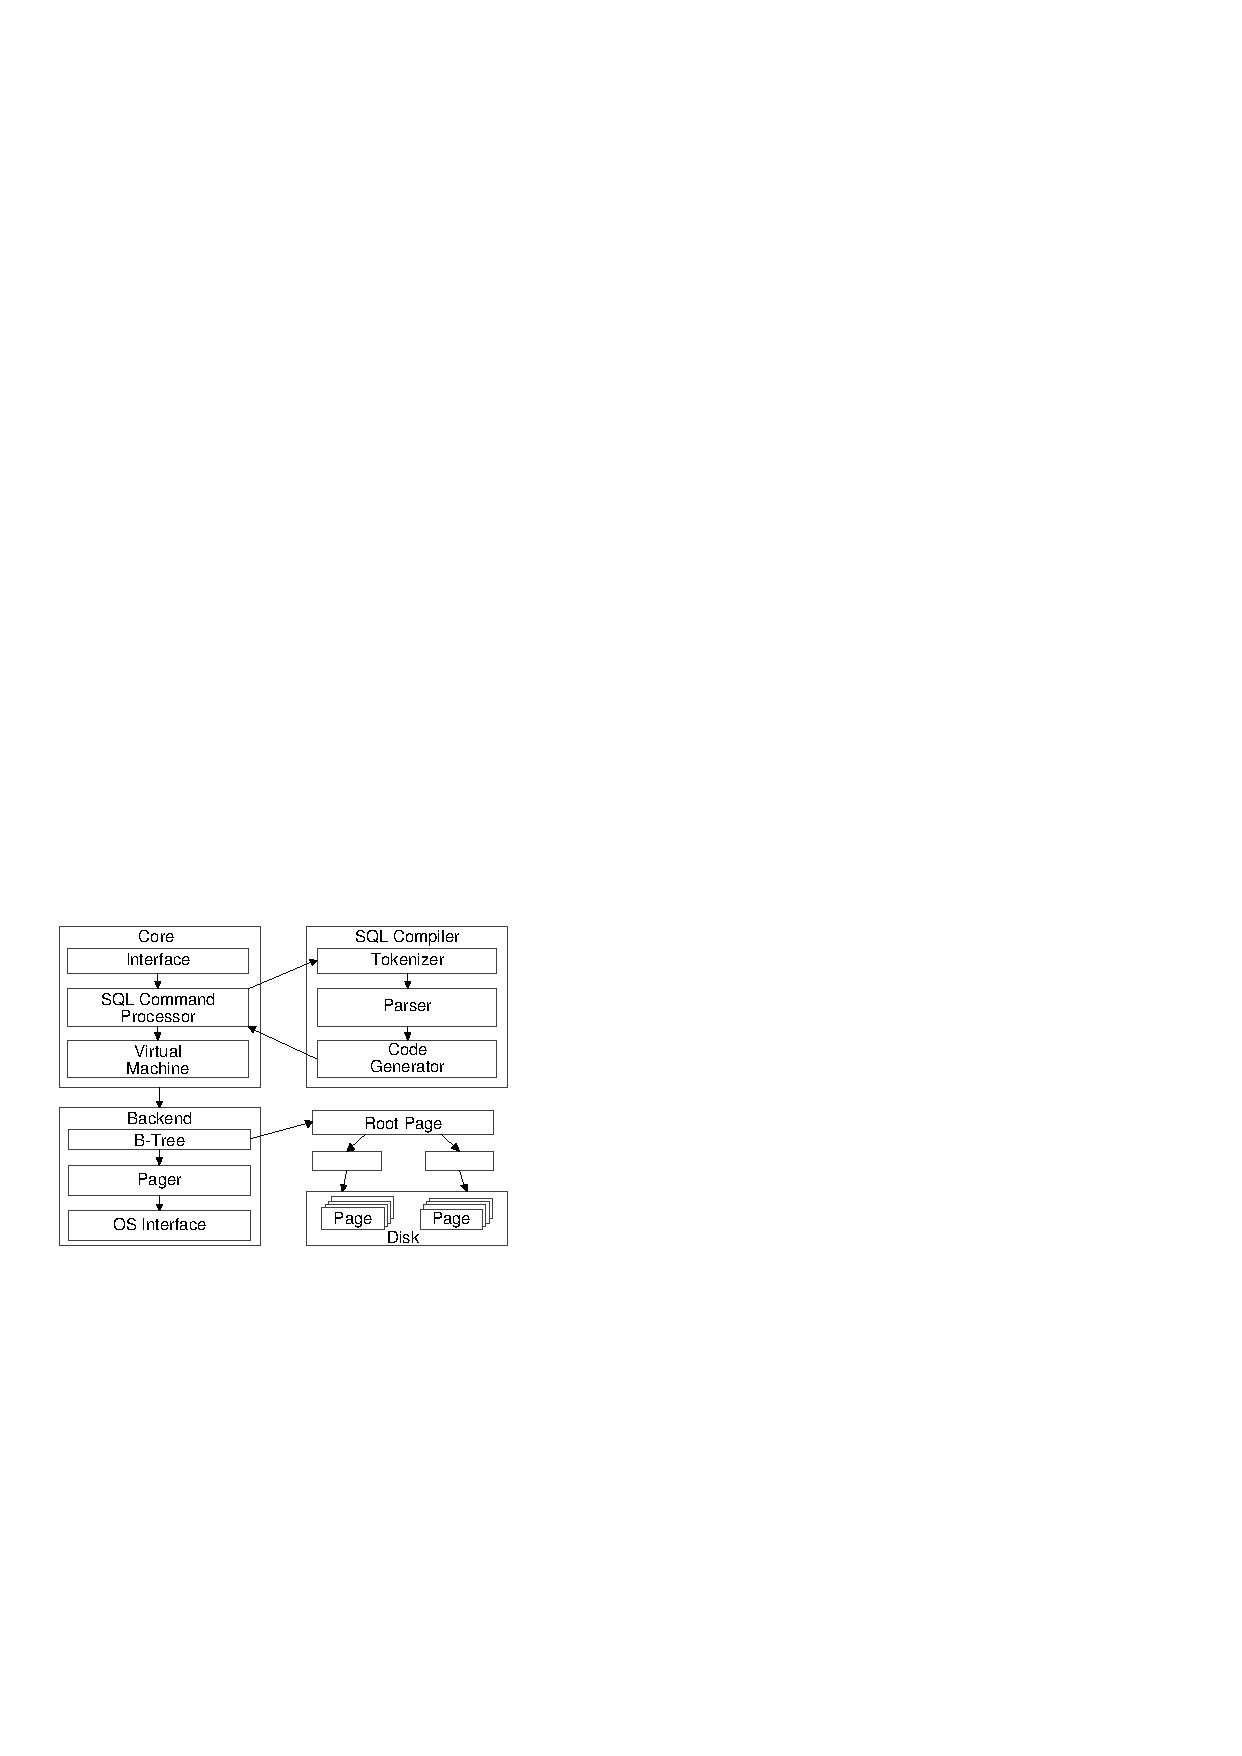
\includegraphics[width=0.5\textwidth]{pic/SQLite.pdf}
		\caption{Architecture of SQLite.}
		\label{fig:SQLite}
	\end{centering}
\end{figure}
SQLite is an in-process library, as well as an embedded SQL database widely used in mobile devices. Figure~\ref{fig:SQLite} gives the architecture of SQLite. SQLite exposes SQL interfaces to applications, and works by compiling SQL statement to bytecode, then running that bytecode using a virtual machine. When compiling one SQL statement, the SQL command processor first send it to the tokenizer. Then Tokenizer breaks the SQL statement into tokens and hands those tokens one by one to the parser. The parser assigns meaning to tokens based on their context, and assembles tokens into a pase tree. After this, the code generator runs to analyze the parser tree and generate bytecode that performs the work of the SQL statement.

The data organization of SQLite database is based B-tree. A separate B-tree is used for each table and index in the database. The B-tree module requests data from the disk in fixed-size pages. The pages can be either table B-tree page, index B-tree page, free page or overflow page. All pages are of the same size and are comprised of multi-byte fields. The pager is responsible for reading, writing, and caching these pages. SQLite communicates with the underlying file system by system
calls like {\tt open}, {\tt write} and {\tt fsync}. Also, SQLite use a journal mechanism for crush recovery, which makes database
file and journal file synchronized frequently with the disk and lead to a performance degradation consequently.


\section{LSM-tree-based Key-Value Database}
\begin{figure}[h]
	\centering
	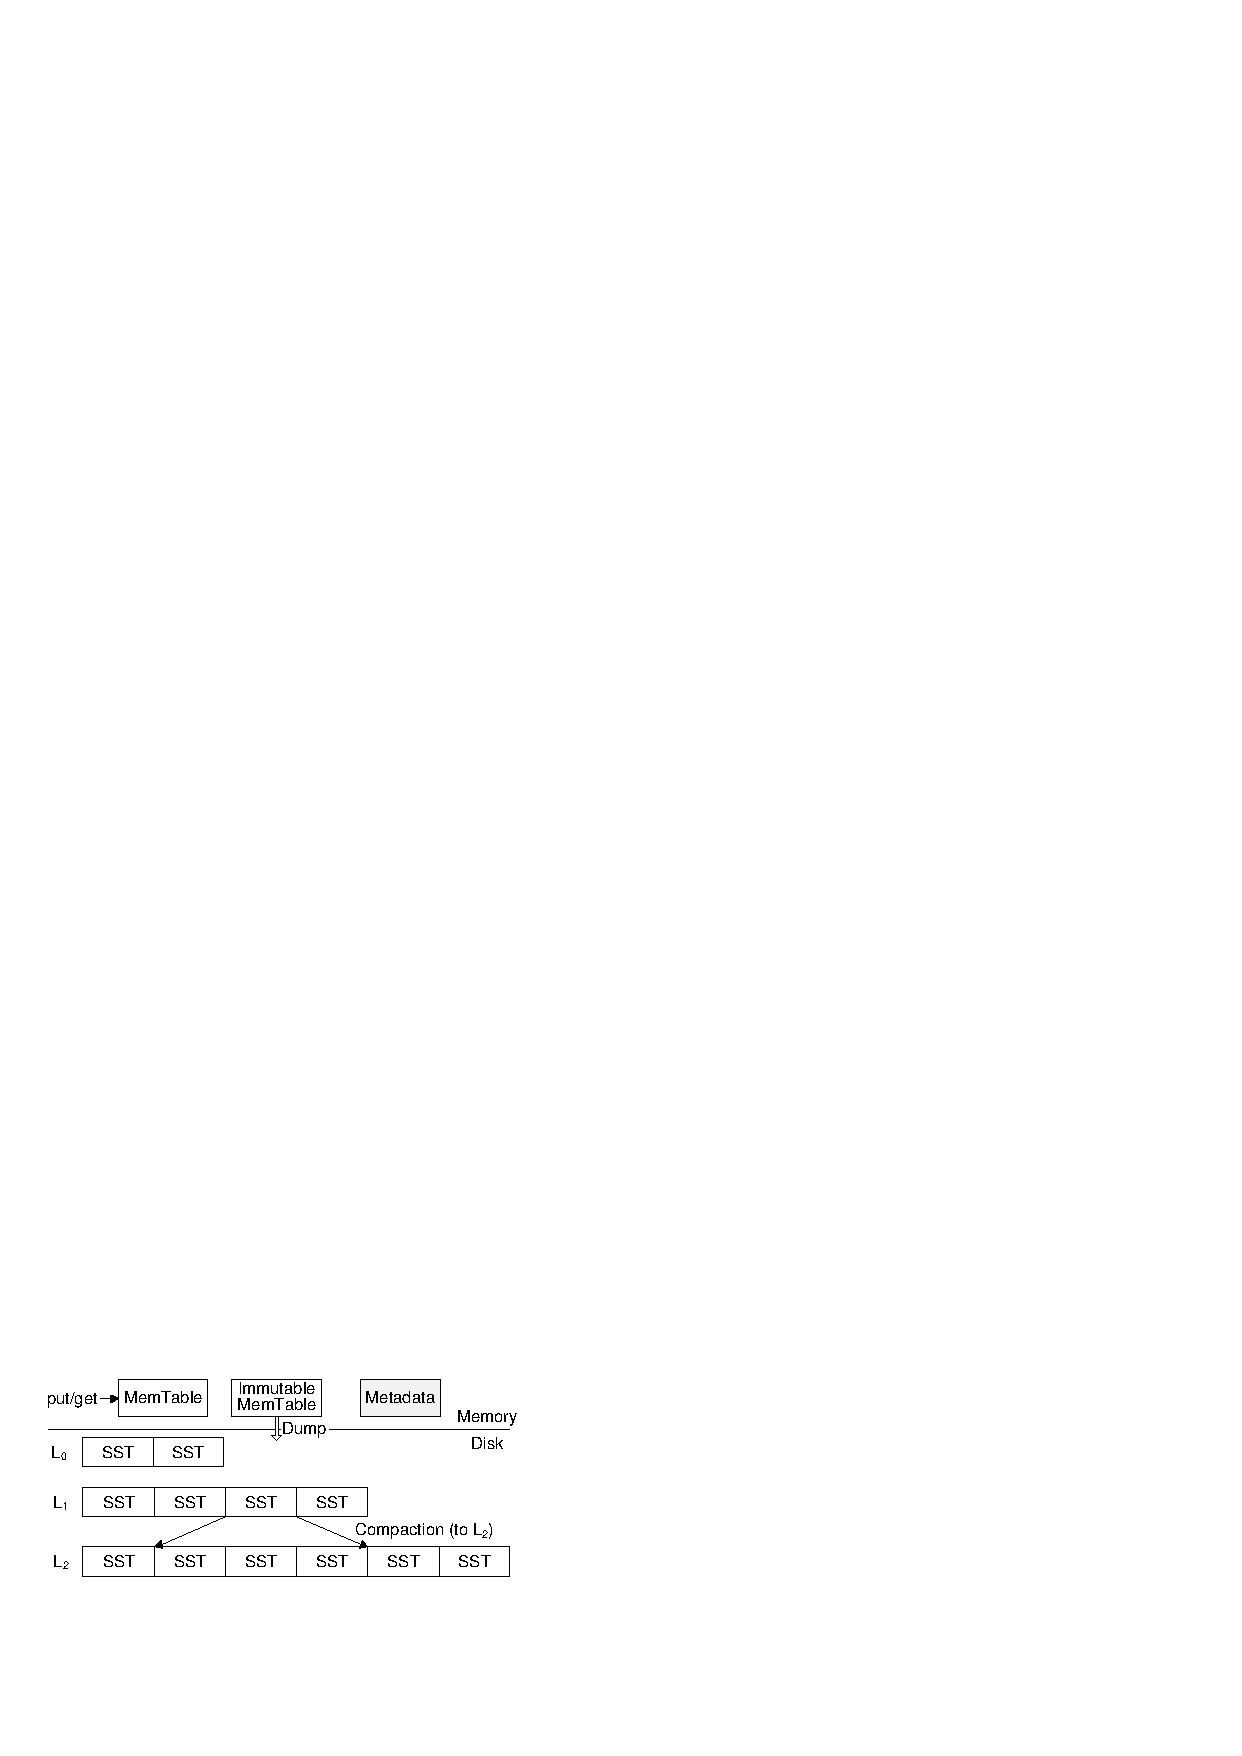
\includegraphics[width=0.5\textwidth]{pic/LSM-TREE.pdf}
	\caption{Architecture of LSM-tree-based Database.}
	\label{fig:LSM-TREE}
	\centering
\end{figure}
A LSM-tree-based key-value database maps a set of keys to the associated values. Applications access their data through simple {\tt SET} and {\tt GET} interfaces.
%We use an embedded LSM-tree-based key-value store SnappyDB~\cite{SnappyDB} to illustrate its working mechanism.
Figure~\ref{fig:LSM-TREE} describes the architecture of an LSM-tree-based key-value database implementation, which consists of two MemTables in main memory and a set of sorted string table (shown as SST in the figure) in the disk. To assist database query operations, meta-data, including indexes, bloom filters, key-value ranges and sizes of these in-disk SSTs are maintained in memory ~\cite{sears2012blsm}.

\begin{figure*}
	\centering
	\begin{minipage}[t]{0.4\textwidth}
		\centering
		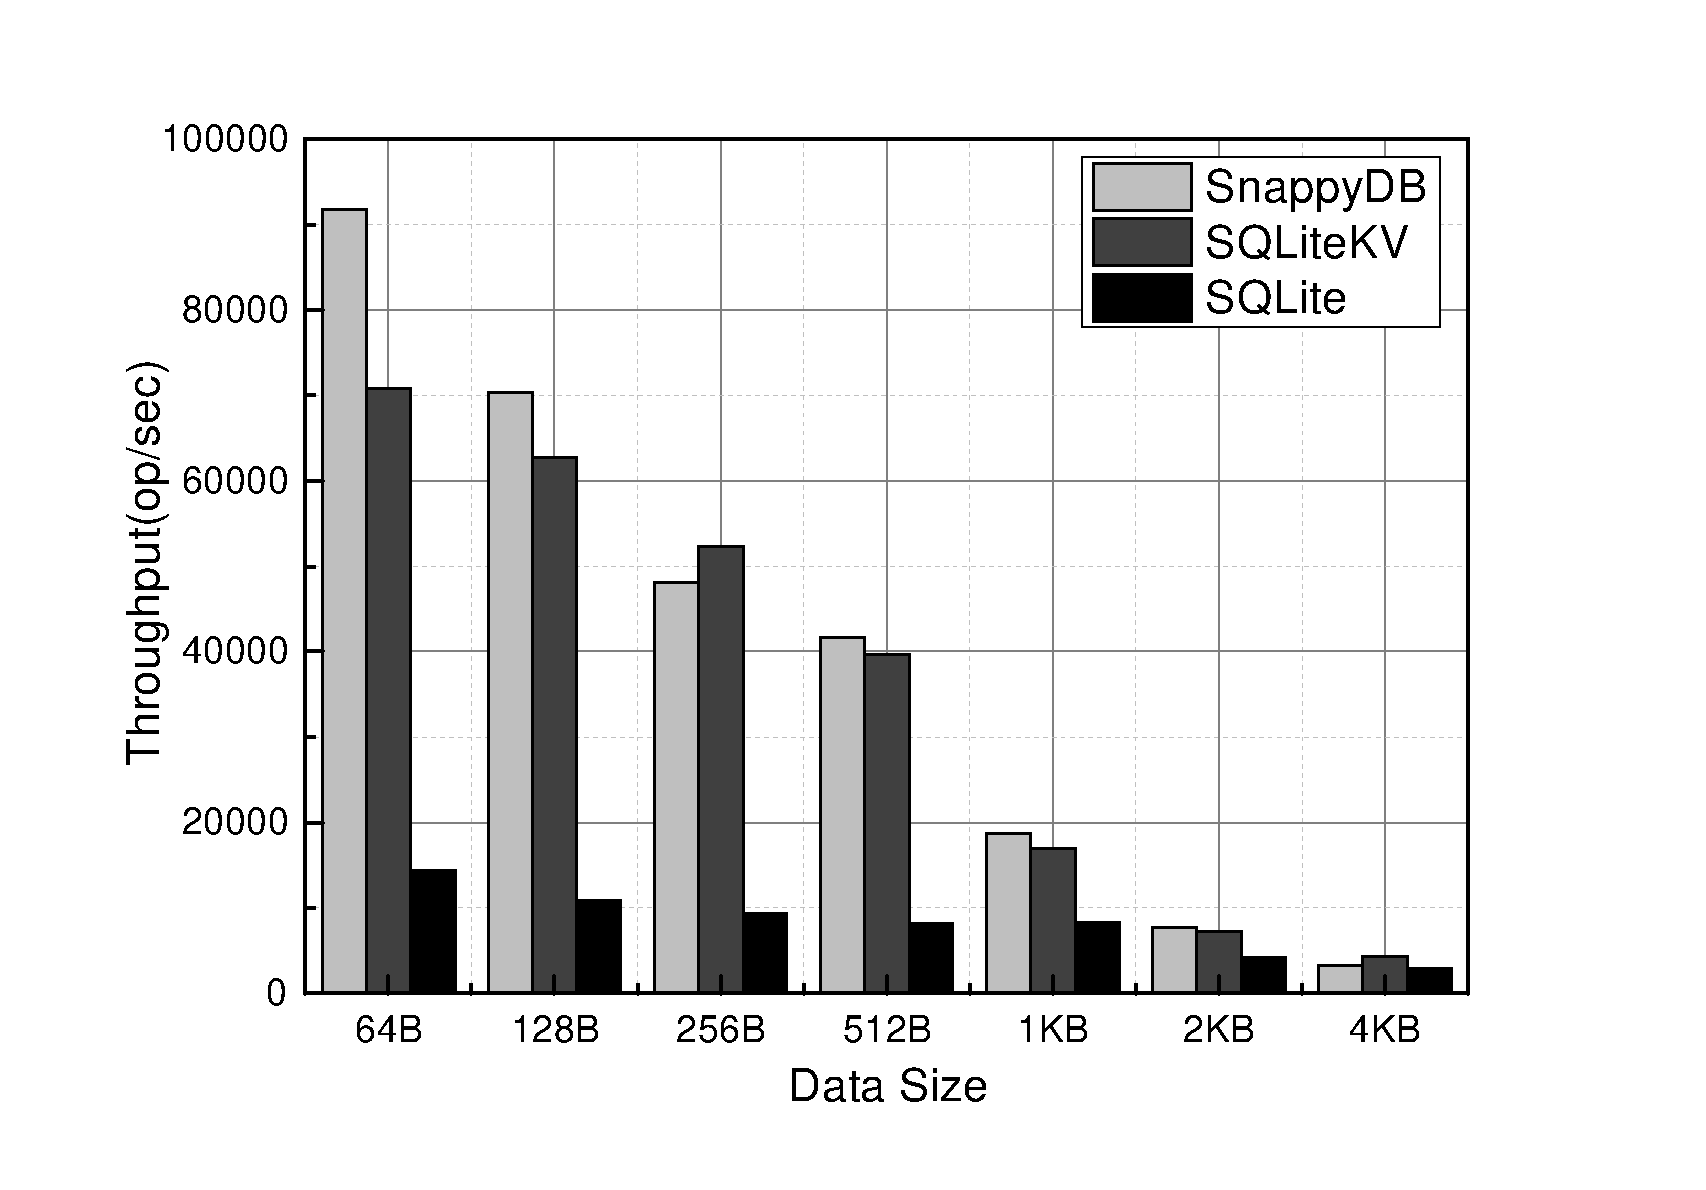
\includegraphics[width=0.95\textwidth]{Ext/workload1.pdf}
		\vspace*{-0.2cm}
		\caption{\small Throughput w. Insert operation.}
		\label{fig:mov_insert}
	\end{minipage}%
	\hspace*{0.7cm}
	\vspace{0.2cm}
	\begin{minipage}[t]{0.4\textwidth}
		\centering
		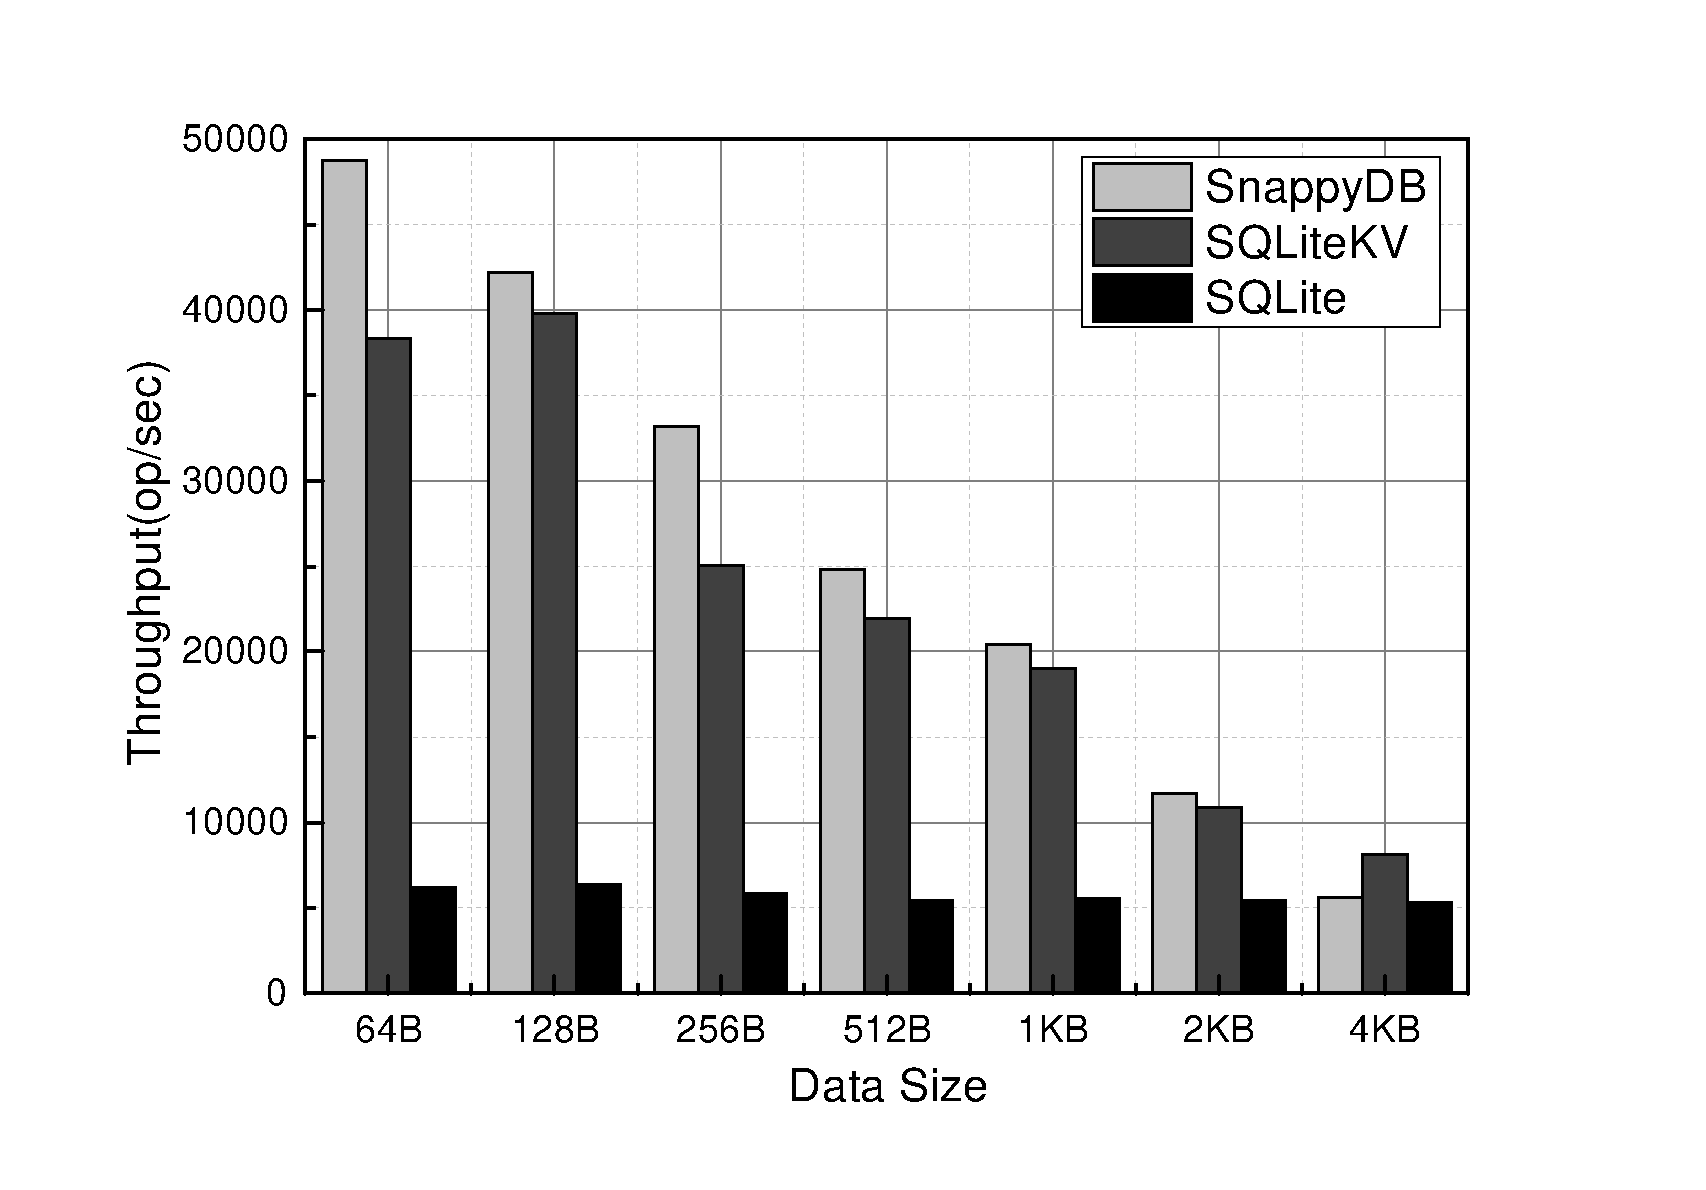
\includegraphics[width=0.95\textwidth]{Ext/workload2.pdf}
		\vspace*{-0.2cm}
		\caption{\small Throughput w. Query operation.}
		\label{fig:mov_query}
	\end{minipage}
	\vspace{0.2cm}
	\caption{\small Performance comparison of SQLite vs SnappyDB}
	\label{fig:motivation}
	\vspace*{-0.3cm}
\end{figure*}


The LSM-tree-based key-value design is based on two optimizations: (1) New data must be quickly admitted into the store to support high-throughput write. The database first use an in-memory buffer, called MemTable, to receive incoming key-value items. Once a MemTable is full, it is transferred into a sorted immutable MemTable, and dumped to disk SSTs. Key-value items in an SSTable are sorted according to their keys. Key range and a bloom filter of each SSTable that are maintained as metadata are cached in memory space to assist key-value search operations. (2) Key-value items in the store are sorted to support fast data location. A multilevel tree-like structure is build to progressively sort key-value items in this architecture. As shown in Figure~\ref{fig:LSM-TREE}, %new SSTables, which are just converted from immutable MemTables, are placed in Level0. 

The youngest level, \emph{Level 0}, is generated by writing the Immutable MemTable from memory to disk. Each level has a limit on the maximum number of SSTables. In order to keep the stored data in an optimized layout, a compaction process will be conducted to merge overlapping key-value items to the next level when the total size of \emph{Level L} exceeds its limit. 



\section{Other SQL-Compatible Key-Value Databases}
Apache Phoenix ~\cite{ApachePhoenix} is an open source SQL skin %relational database 
which receives SQL query by compiling it into a series of key-value operations of Apache HBase, a distributed, key-value, big data store. Phoenix provided a well-defined and industry standard APIs for OLTP and operational analytics for Hadoop. Nevertheless, without a deep integration with Hadoop framework, it is difficult for mobile devices to adopt either HBase as its storage engine or Phoenix for SQL-to-KV transitions. Besides, Phoenix, along with other Hadoop-related modules, is designed for scalable and distributed computing environments with large data sets ~\cite{forman1994challenges}, which means they can hardly fit in mobile environments as a matter of durability, battery life and portability ~\cite{sinha2016low}.

In this paper, we propose an efficient LSM-tree-based lightweight Database engine, SQLiteKV, which retains SQLite interface for mobile devices, keeps a high performance compared with SQLite and adopt an efficient LSM-tree structure on its storage engine.


 \chapter{Project Methodology}
\label{chap:Methodology}
In this section, we present SQLiteKV and its detailed design architecture. SQLiteKV is a variant of LSM tree-based key value storage engine, like Google's LevelDB or Facebook's Cassandra. It is augmented with two layers and four modules. The front-end layer includes a SQL-to-KV compiler, from which existing applications could migrate from SQLite to key-value storage without any modifications on their original SQLite codes, as well as a slab-allocation caching for memory efficiency and de-fragmentation. At the back-end layer of SQLiteKV, a new index management scheme is proposed to work along with the underlying LSM-tree-based storage engine. It can significantly improve the performance and scalability of meta-data management as well. 

\section{Design Overview}
\begin{figure}[h]
	\centering
	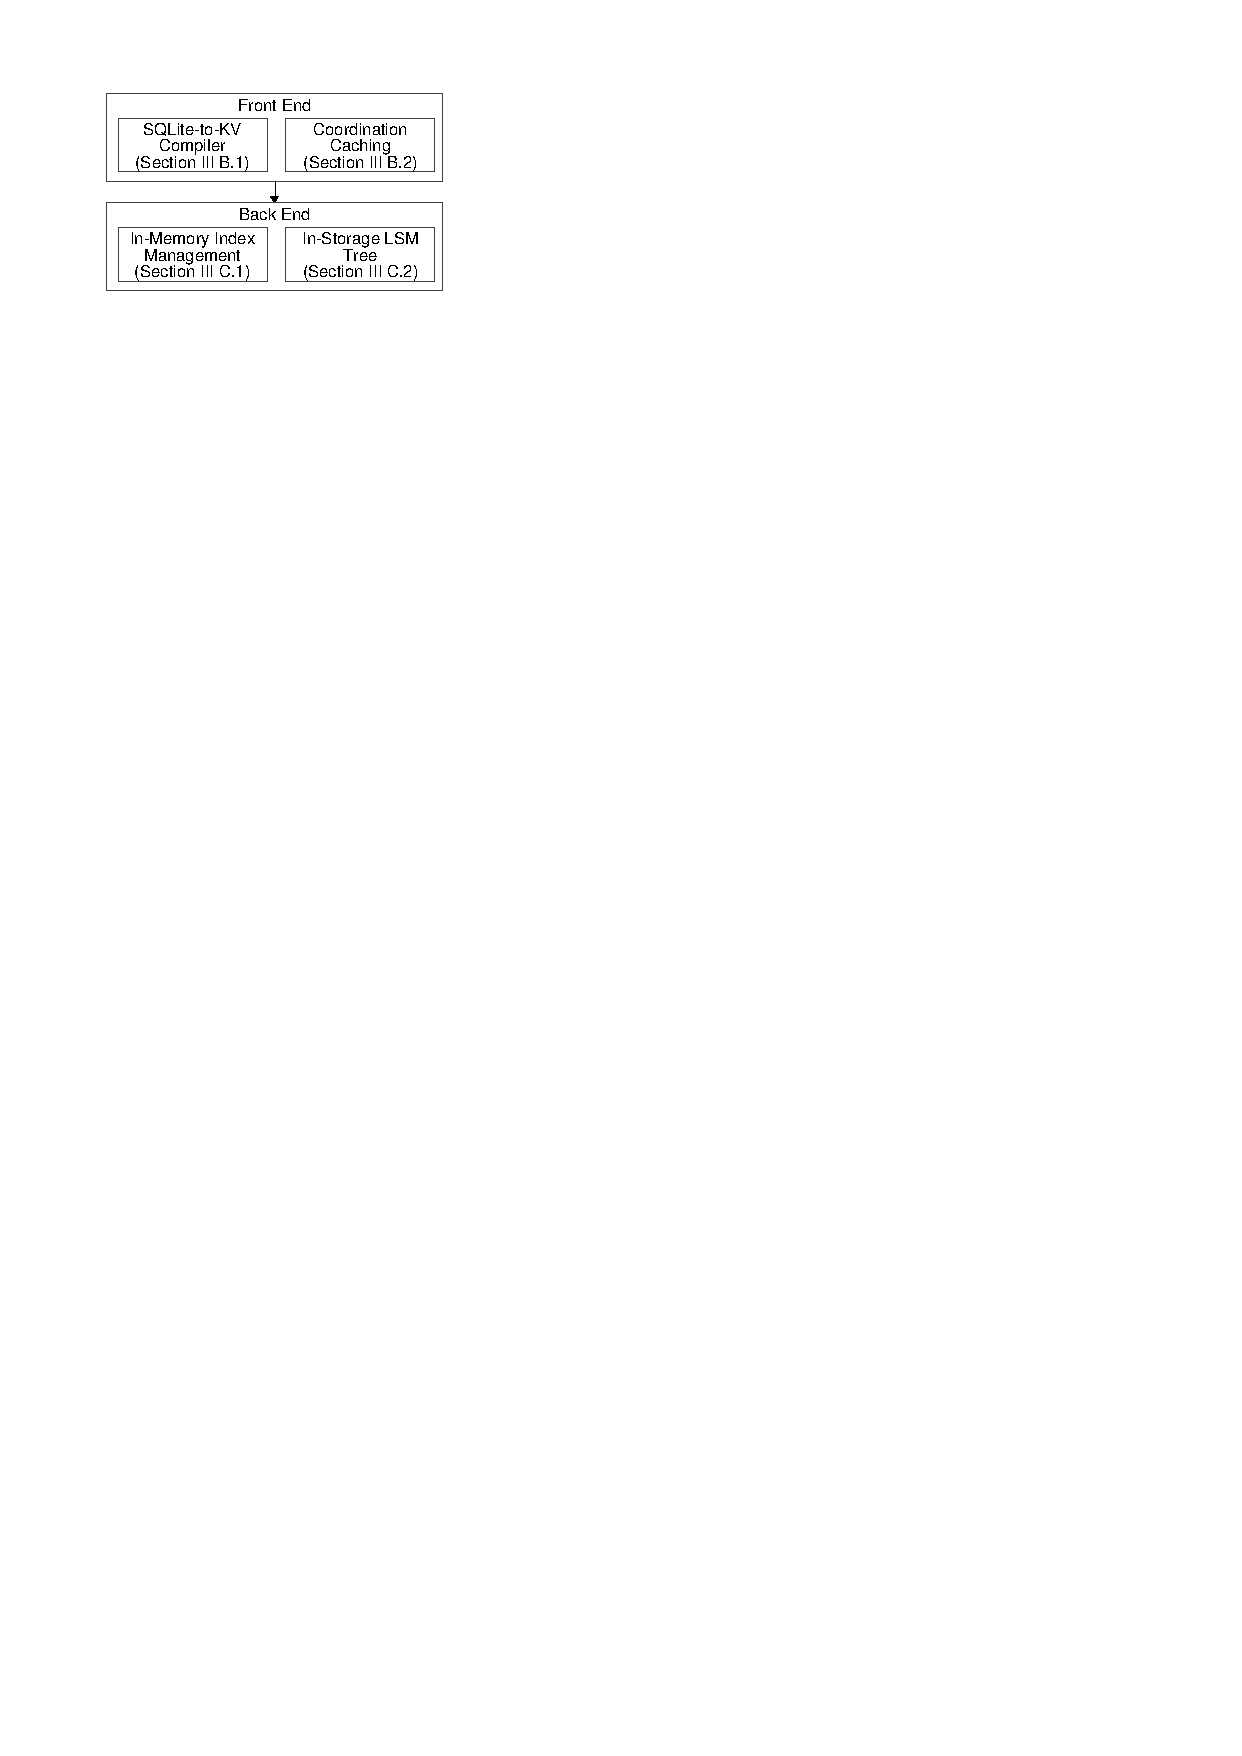
\includegraphics[width=0.4\textwidth]{pic/SQLiteKV.pdf}
	\caption{Architecture of SQLiteKV.}
	\label{fig:SQLiteKV}
	\centering
\end{figure}
As shown in Fig ~\ref{fig:SQLiteKV}, SQLiteKV is augmented with two layers, the front-end layer and the back-end layer. Front-end layer consists of two modules: a SQLite to KV compiler and a slab-allocation caching. As energy optimization is of vital importance in mobile devices and memory contributes to a large portion of total energy consumption of embedded devices \cite{shao2012utilizing},  our back-end layer  mainly focus on the memory and storage optimization. The two main modules of it are a re-designed index management and a LSM-tree based storage engine. 

The overall architecture and these functional modules are illustrated in Figure~\ref{fig:SQLiteKV}.  The two layers with four functional modules are described below in more details.
\subsection{Front-End}
	In order to provide a SQLite-Compatible interface, two major components are designed and implemented on the front-side of SQLiteKV. Fig ~\ref{fig:SQLite2KVCompiler} shows the first one-a SQLite-like interface and the second one, a slab-allocation caching mechanism, is presented in Fig ~\ref{fig:cache}.
	\subsubsection{SQLite-Like Compiler}
	\begin{figure}[h]
		\centering
		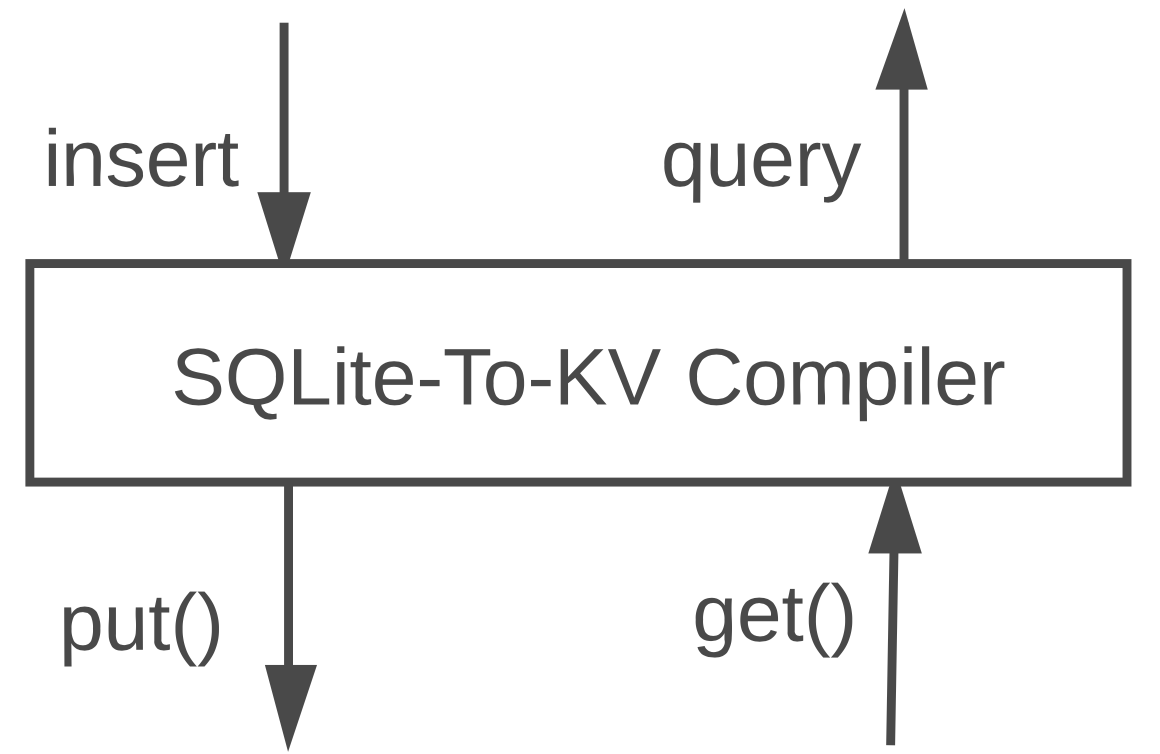
\includegraphics[width=0.35\textwidth]{pic/SQLite2KV.png}
		\caption{SQLite to KV Compiler work flow.}
		\label{fig:SQLite2KVCompiler}
		\centering
	\end{figure}
 	As for the interpretation of SQL statements, our SQLite-to-KV compiler firstly breaks down the statements into tokens. Then it would give each token meaning based on the context and assemble it into a parser tree. So far the compilation goes similarly as SQLite. The most important step is that it would generate key-value operations based on the result of parsing. Generally, there would be three kind of operations including GET(), PUT()  and DELETE(), which is also a common feature among NoSQL database. KV operations will be passed to and executed in the back-end storage engine.
	
	This SQLite-to-KV compiler makes it possibile that existing applications could run smoothly with original SQL statements and leverage the potentials of key value storage.
	
	\subsubsection{Slab-Allocation Caching}
		\begin{figure}
		\centering
		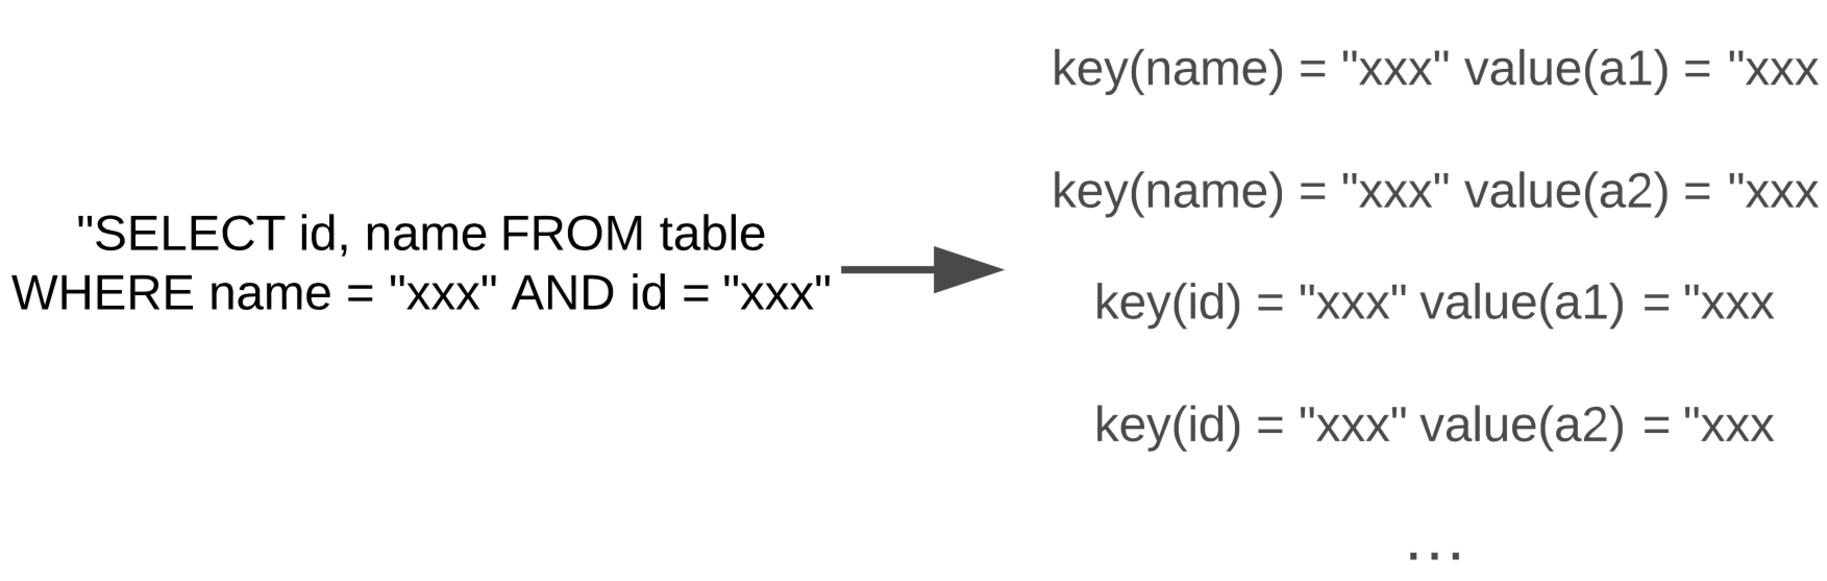
\includegraphics[width=0.6\textwidth]{pic/Cache-eg.pdf}
		\caption{One Single SQL to Multi KV items.}
		\label{fig:CacheEG}
	\end{figure}
		\begin{figure}[h]
			\centering
			\begin{subfigure}[b]{0.35\textwidth}
				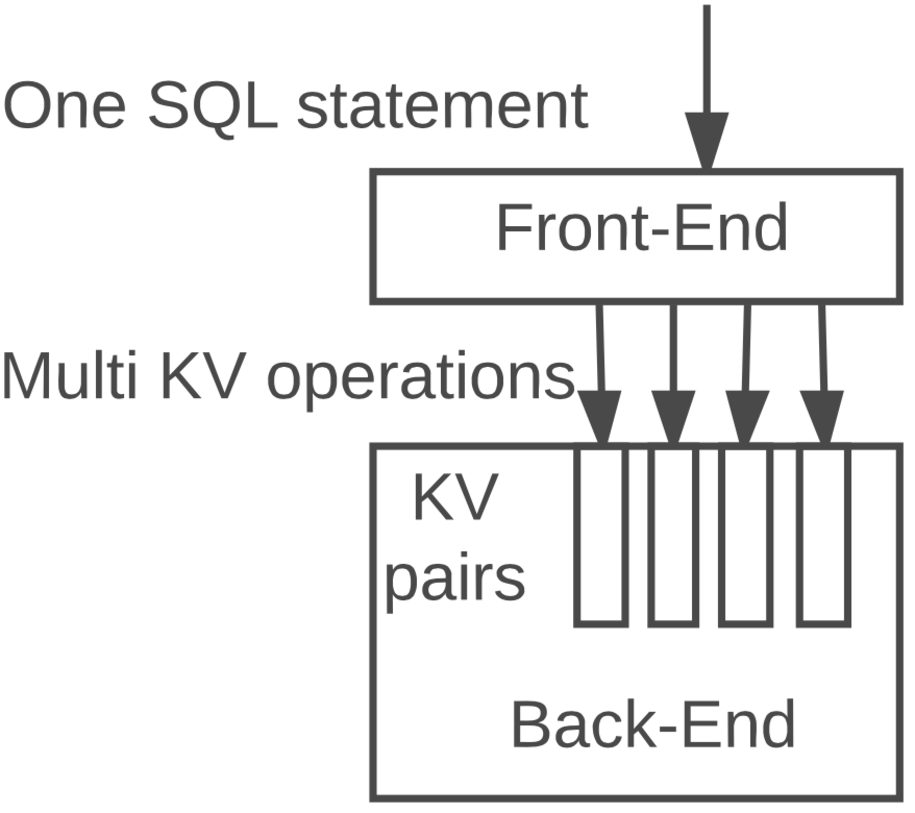
\includegraphics[width=\textwidth]{pic/KVCache.pdf}
				\caption{SQLiteKV without Cache.}
				\label{fig:KVCache}
			\end{subfigure}
		\begin{subfigure}[b]{0.35\textwidth}
			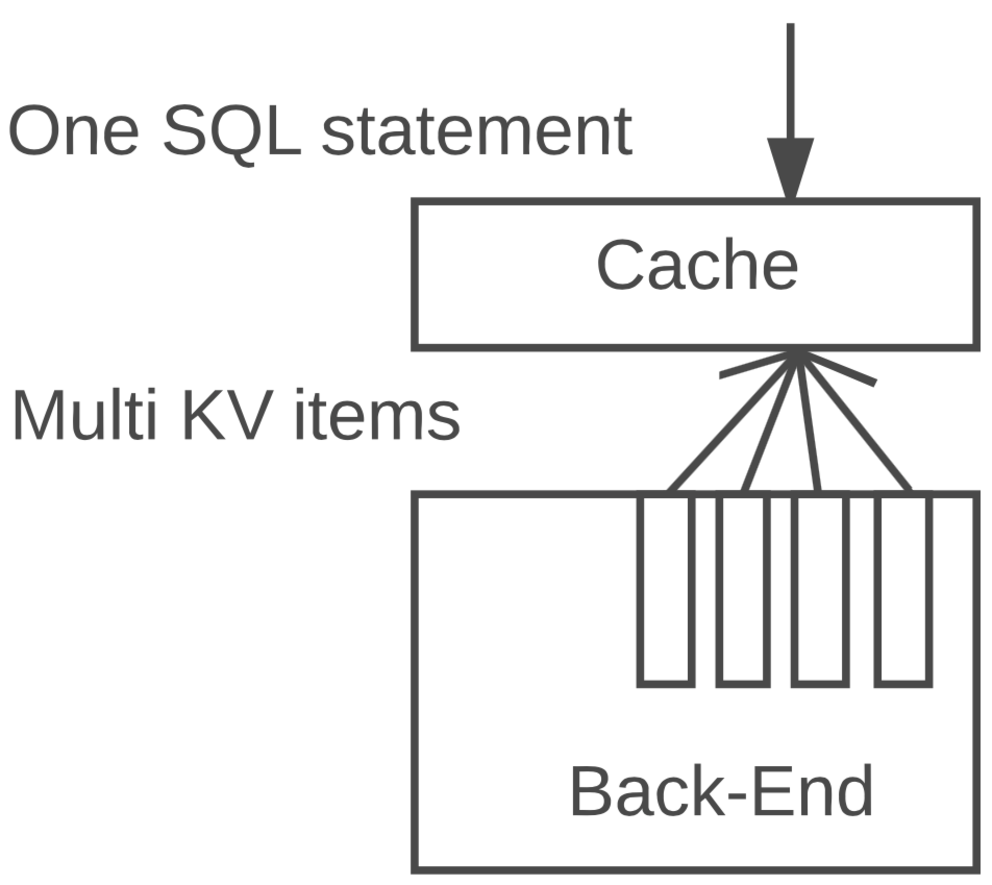
\includegraphics[width=\textwidth]{pic/SQLiteKVCache.pdf}
			\caption{SQLiteKV with Cache.}
			\label{fig:SQLiteKVcache}
		\end{subfigure}
	\caption{SQLite Slab-Allocation Caching}
	\label{fig:cache}
	\end{figure}
	 SQLite uses a caching mechanism inside its back end engine to cache frequently-visited pages within the flash memory to avoid frequent visits to the disk. SnappyDB also implements a caching system for latest recently used KV items. However, one SQL statement usually corresponds to multi-KV items during the SQL compilation process of SQLiteKV. Neither of these above-mentioned caching could alleviate such data discrepancy between SQL statements and KV items. Therefore, we design a new caching mechanism as part of the front-end of SQLiteKV. It caches query results for SQL statements as a batch of KV items. Such mapping between SQL statement and KV items can significantly reduce the data discrepancy and improve the query performance.
	 \begin{figure}
	 	\centering
	 	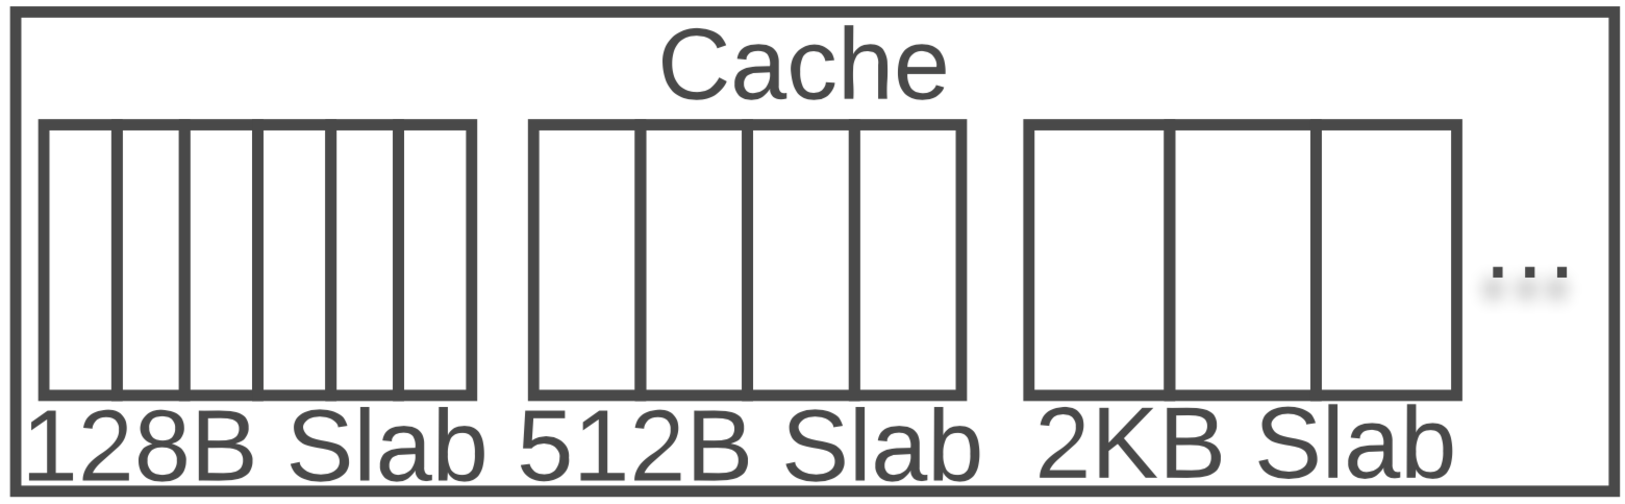
\includegraphics[width=0.3\textwidth]{pic/SQLiteKVCache2.pdf}
	 	\caption{SQLiteKV Cache Structure.}
	 	\label{fig:SQLiteCache2}
	 	\centering
	 \end{figure}
	 Moreover, a slab-allocation structure, as shown in Fig. \ref{fig:SQLiteCache2} is deployed to solve the memory fragmentation issue caused by small KV items. The slab-based caching mechanism would separate memory space into different slabs with various entry sizes, like 128 bytes, 512 bytes or 4096 bytes. A specific KV item would be cached into a slab whose size fits the itself the most. Such design can effectively address the issue of memory fragmentation, especially on embedded memory constraints devices.

\subsection{Back-End}
	\subsubsection{Index Management On LSM Tree}

 	LSM-based storage engines would commonly do a scan over the entire disk and collect all indexes back to the memory \cite{190528}. Usually index is put at the end of each data block. Hence when a query operation is to be executed, the in-memory meta-data would be binary-searched with the target key to locate the data block on disk. That data block would be visited upon then which means at most one disk seek is required for a single query on LSM-tree-based KV engine. 
 			\begin{figure}
 		\centering
 		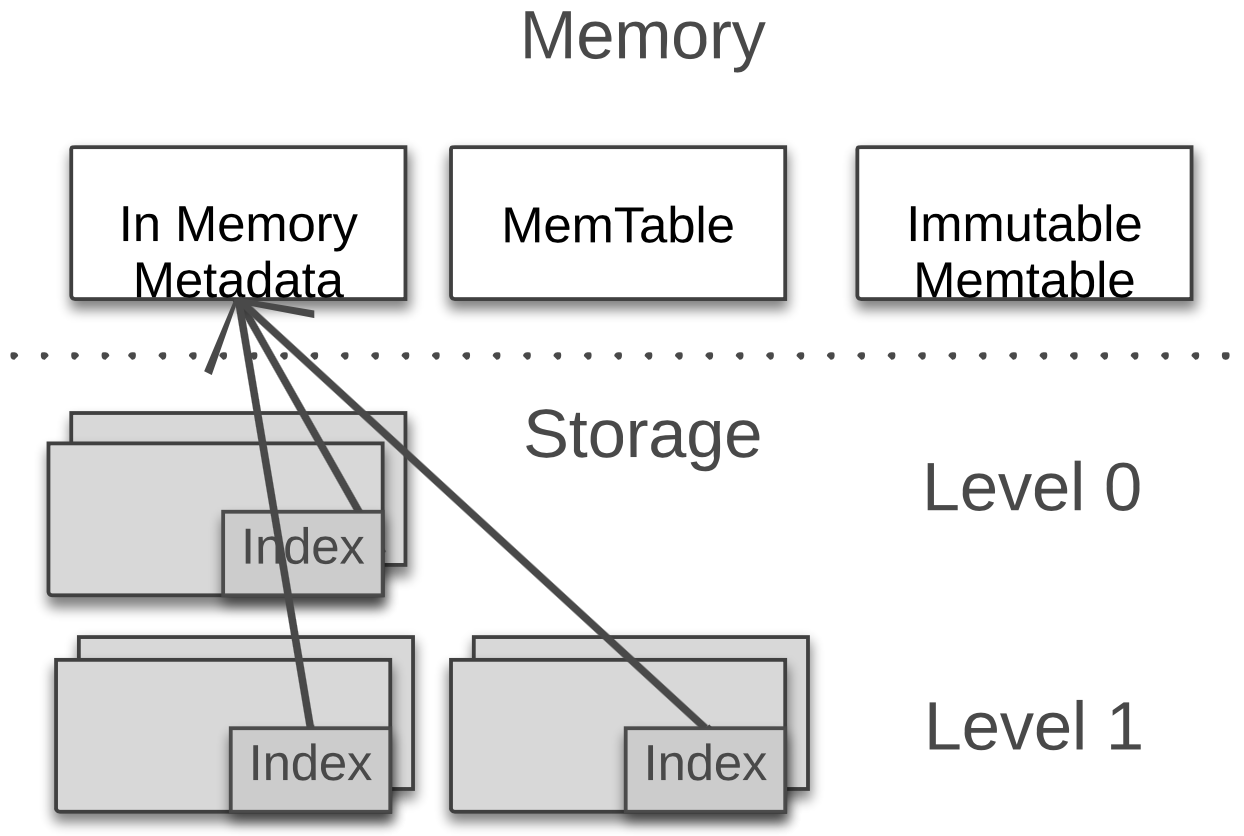
\includegraphics[width=0.35\textwidth]{pic/Back-Index.png}
 		\caption{Back-End In-Memory Index Management.}
 		\label{fig:back-index}
 		\centering
 	\end{figure}
 	However, this approach doesn't seem to be practical nor efficient since most mobile devices are memory constraints and not all the indexes could be accommodated in the memory. In accordance to this issue, we re-design the indexing management scheme, which exclusively stores indexes of data blocks in higher levels, like level 0 and 1, of the entire LSM tree. The reason is that with the level goes further down, data at lower level are less likely to be visited. In other words, the data on top levels are more likely to be newly-added or frequently-visited. Our approach reduce the huge overhead on SnappyDB's original in-memory meta-data management. At the same time, the worst disk seek time remains at same order of complexity. To sum up, our meta-data management strategy does leverage the LSM-tree structure and avoid possible memory constraints issue on the back-end side.
	
	\subsubsection{Storage Management}
		\begin{figure}[h]
		\centering
		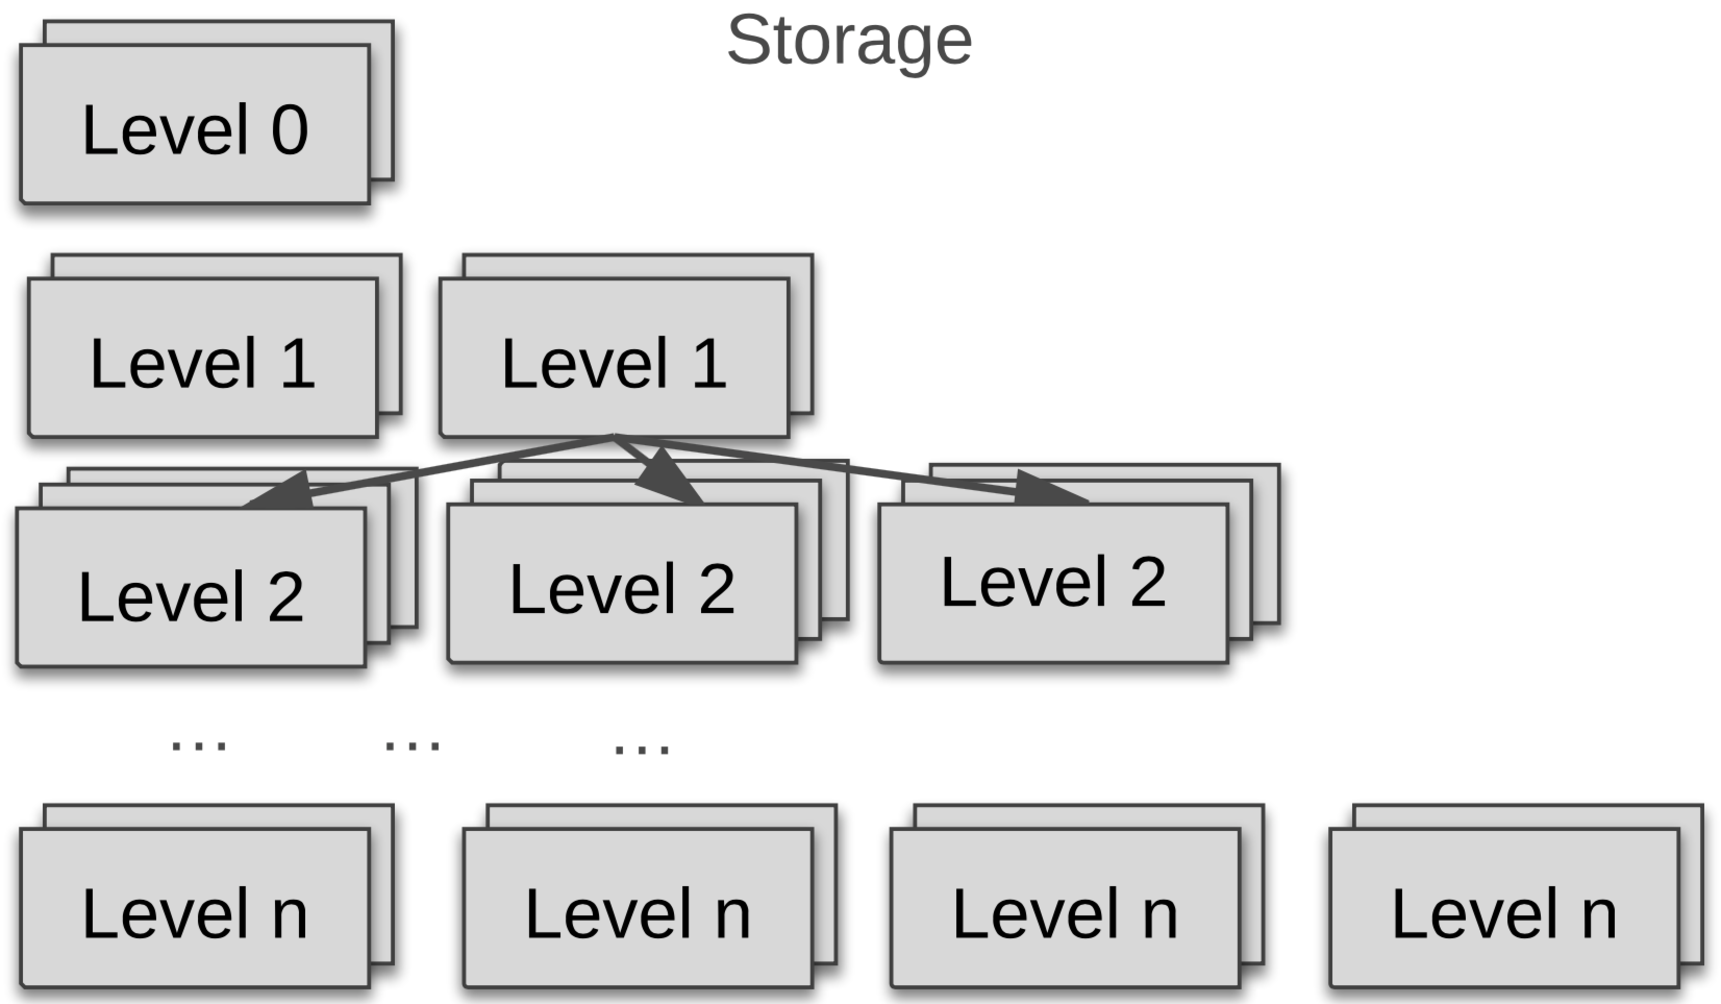
\includegraphics[width=0.32\textwidth]{pic/Back-Disk.pdf}
		\caption{Back-End Storage Management.}
		\label{fig:BackDisk}
		\centering
	\end{figure}

	The disk storage management of SQLiteKV relies mainly on its LSM-tree-based structure. As we mentioned before, once the MemTable, as shown in Fig ~\ref{fig:back-index}, is converted to be an immutable table and dumped into disk. This SSTable would be placed at the first level, level 0. As long as one specific level of this LSM tree is full, those SSTables with overlapping indexes would be compacted together and dumped to the next level. During this compaction process, newly-generated SSTables on lower levels tend to have larger  sizes and ranges of index consequently. 


 \chapter{Evaluation}
\label{chap:Results}

This section presents the evaluation results by comparing SQLiteKV with SQLite and SnappyDB, which are representative SQL and Key-value databases, respectively. In this section, we first introduce the experimental setup, then provide the experimental results with real-world benchmarks and synthetic workloads, with the overhead analysis provided at the end \cite{cooper2010benchmarking}.
\section{Experiment Setup}
We have prototyped the proposed SQLiteKV on Google Nexus platform. Our implementation is based on SQLite and SnappyDB, and includes 2,344 lines of code. 

All experiments have been conducted on Google’s Nexus 6p smartphone that has a 2.0 GHz oct-core 64 bit Qualcomm Snapdragon 810 processor, 3 GB LPDDR4 RAM, Samsung-manufactured 32 GB eMMC 5.0 NAND flash and Android 7.1.2 with Linux Kernel 3.10.73.

SQLite 3.9 is utilized in the experiments as this is the current version in Google Nexus 6p. The page size of SQLite is set as 1024 bytes that is the default valud. SnappyDB 0.4.0 is adopted that is the latest version of a java implementation of Google's LevelDB. SQLiteKV is implemented based on the same version of SnappyDB. 

To make a fair comparison, in our experiments, for each SQL query in SQLite, it contains up to 999 variables that is the maximum value allowed. In this way, we avoid unnecessary inefficiency from one benchmark tool ~\cite{SnappyDB} from SnappyDB in which one SQLite query would only carry one variable at one time. Moreover, unnecessary calls like cursor.moveToFirst() after queries are not performed for the sake of efficiency.

\section{Overall Performance}

%To generate real-world key-value requests to the database engine, we adopt a workload model presented in prior work \cite{shen2017didacache}. This model is built based on real workloads \cite{atikoglu2012workload}, and 
Based on the database benchmark tool \cite{cooper2010benchmarking}, we have generated a set of real-world workloads to evaluate the overall performance. The ratio of insertions and queries of each workload is shown in Table ~\ref{table:workload}.
\begin{table}
	\begin{center}
		\caption{Workload  Characteristics.}
		\begin{tabular}{|p{2.5cm}|p{1.5cm}|p{1.5cm}|} 
			\hline
			Workload(s) & Query & Insert \\ 
			\hline
			Update Heavy & 0.5 & 0.5 \\ 
			\hline
			Read Most & 0.95 & 0.05 \\
			\hline
			Read Heavy & 1 & 0 \\
			\hline
			Read Latest & 0.05 & 0.95  \\ 
			\hline
		\end{tabular}
		\label{table:workload}
	\end{center}
\end{table}

To generate real-world requests to the database engines, we first generate 100 thousand key value pairs to populate our databases, and then use the object popularity model to generate 100 thousand SQLite and KV requests, respectively. The object popularity, which determines the request sequence, follows a Zipfian distribution ~\cite{shen2017didacache}, by which some records in the head will be extremely popular while some in the tail are not. In the Read Latest workload, it follows the Zipfian distribution except that most recently inserted records will be in the head of the distribution so they will be accessed more frequently. For all other workloads, record selections follow Zipfian distribution. 
\begin{figure*}
	\centering
	\begin{minipage}[t]{0.4\textwidth}
		\centering
		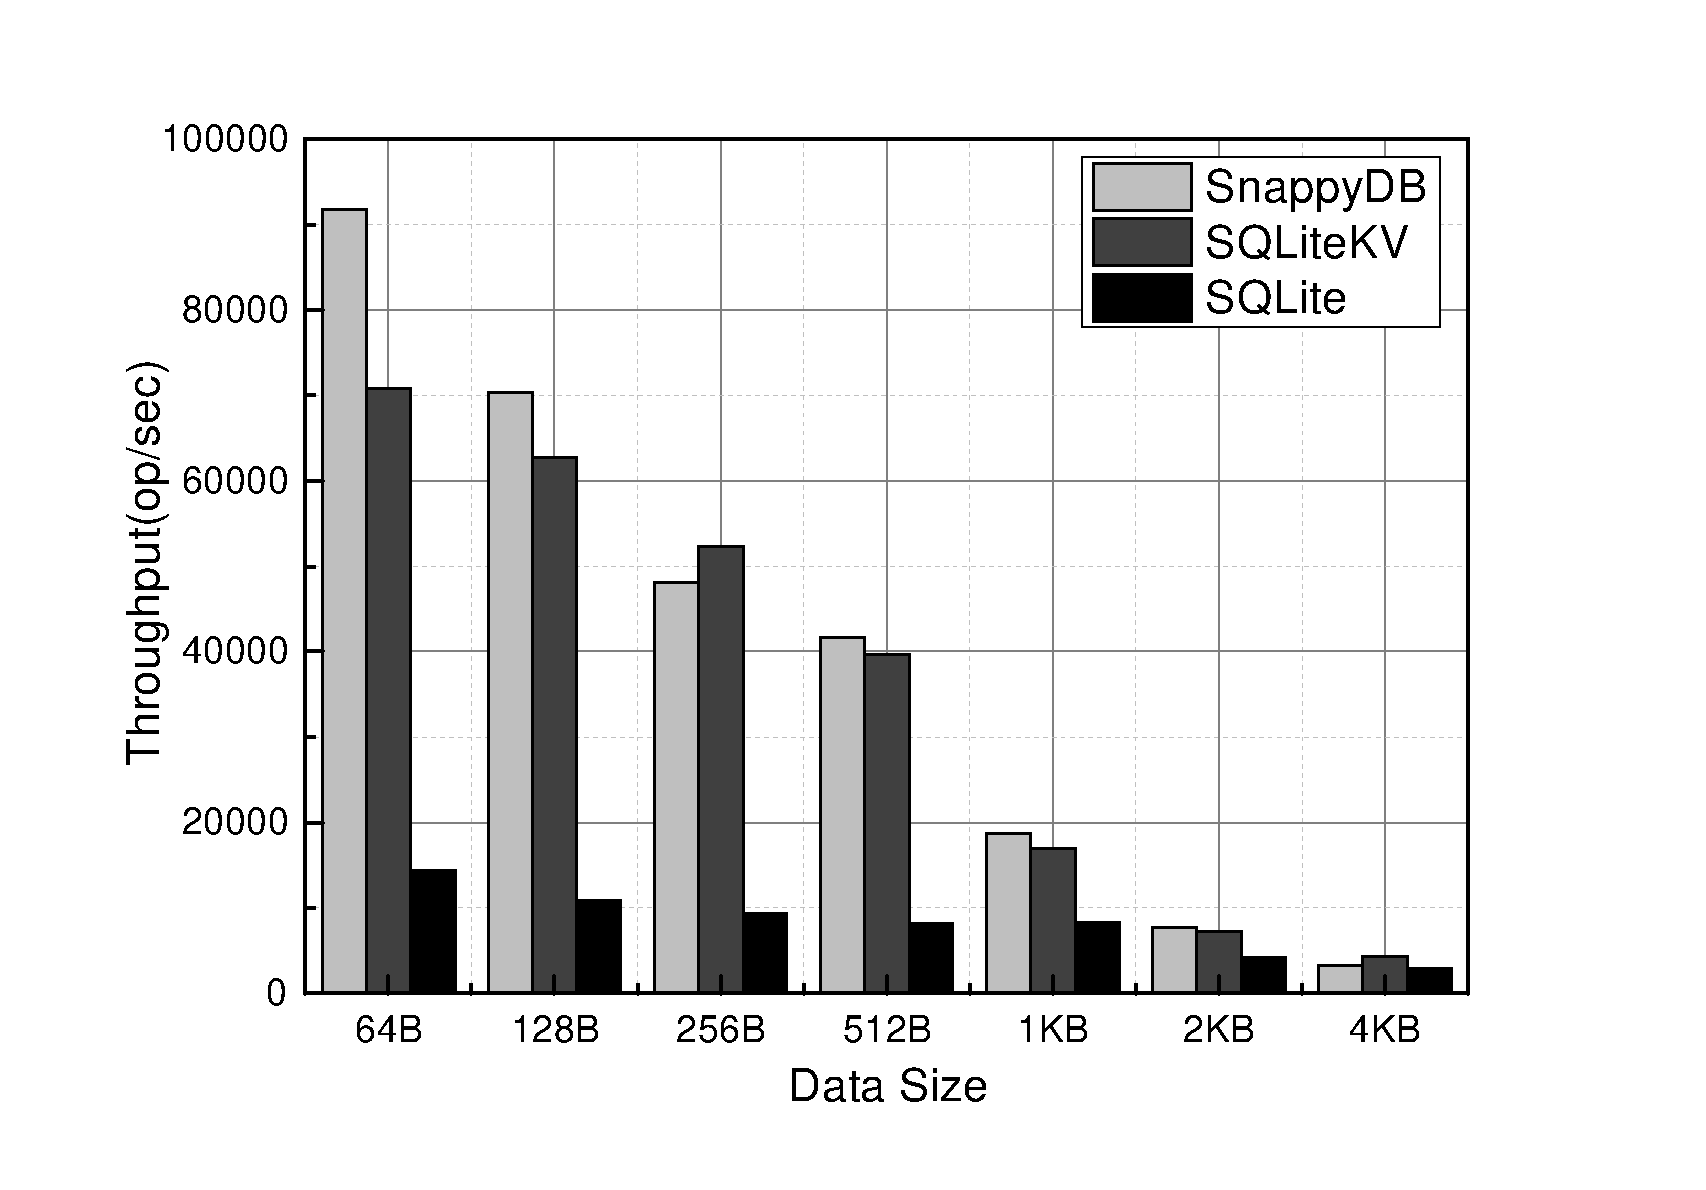
\includegraphics[width=0.9\textwidth, height=3.5cm]{Ext/workload1.pdf}
		\vspace*{-0.2cm}
		\caption{\small Throughput w. Update Heavy Workload.}
		\label{fig:workload1}
	\end{minipage}%
	\hspace*{0.7cm}
	\begin{minipage}[t]{0.4\textwidth}
		\centering
		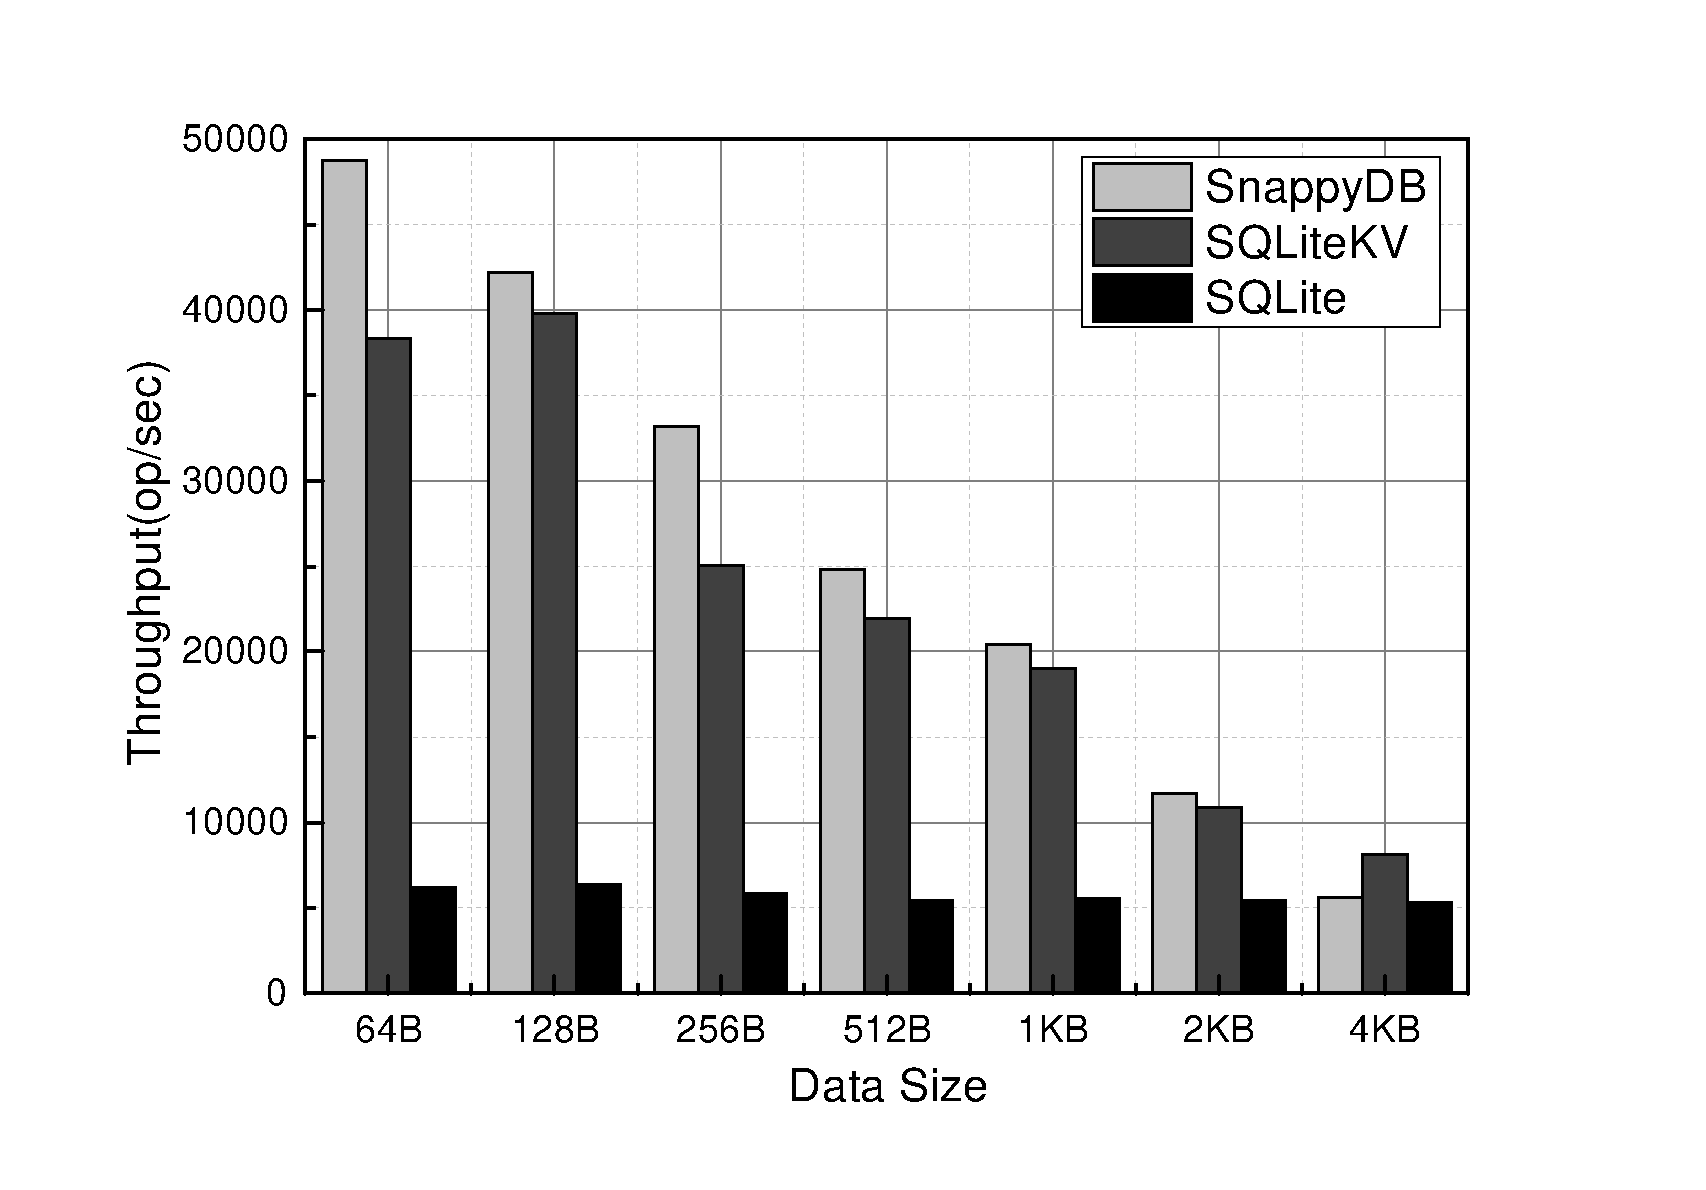
\includegraphics[width=0.9\textwidth, height=3.5cm]{Ext/workload2.pdf}
		\vspace*{-0.2cm}
		\caption{\small Throughput w. Read Most Workload.}
		\label{fig:workload2}
	\end{minipage}
\end{figure*}

\begin{figure*}
	\centering
	\begin{minipage}[t]{0.4\textwidth}
		\centering
		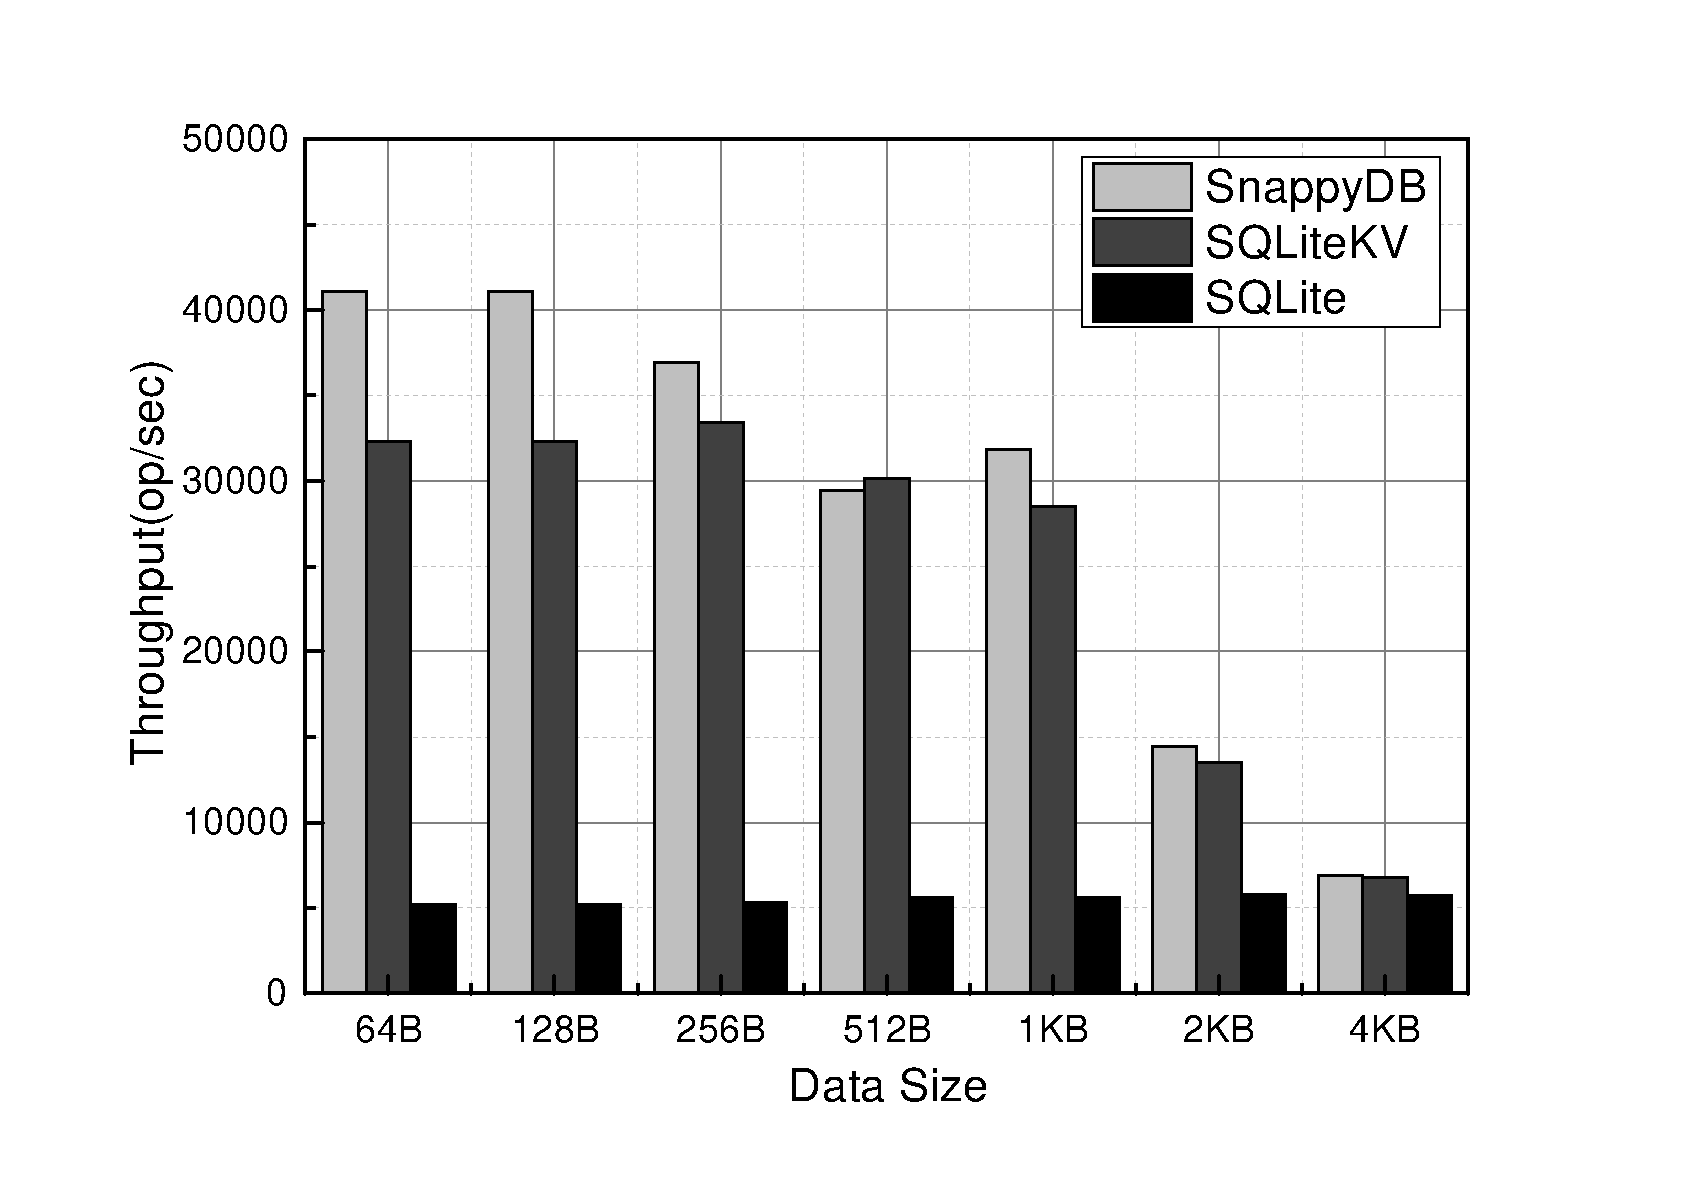
\includegraphics[width=0.9\textwidth, height=3.5cm]{Ext/workload3.pdf}
		\vspace*{-0.2cm}
		\caption{\small Throughput w. Read Heavy Workload.}
		\label{fig:workload3}
	\end{minipage}%
	\hspace*{0.7cm}
	\begin{minipage}[t]{0.4\textwidth}
		\centering
		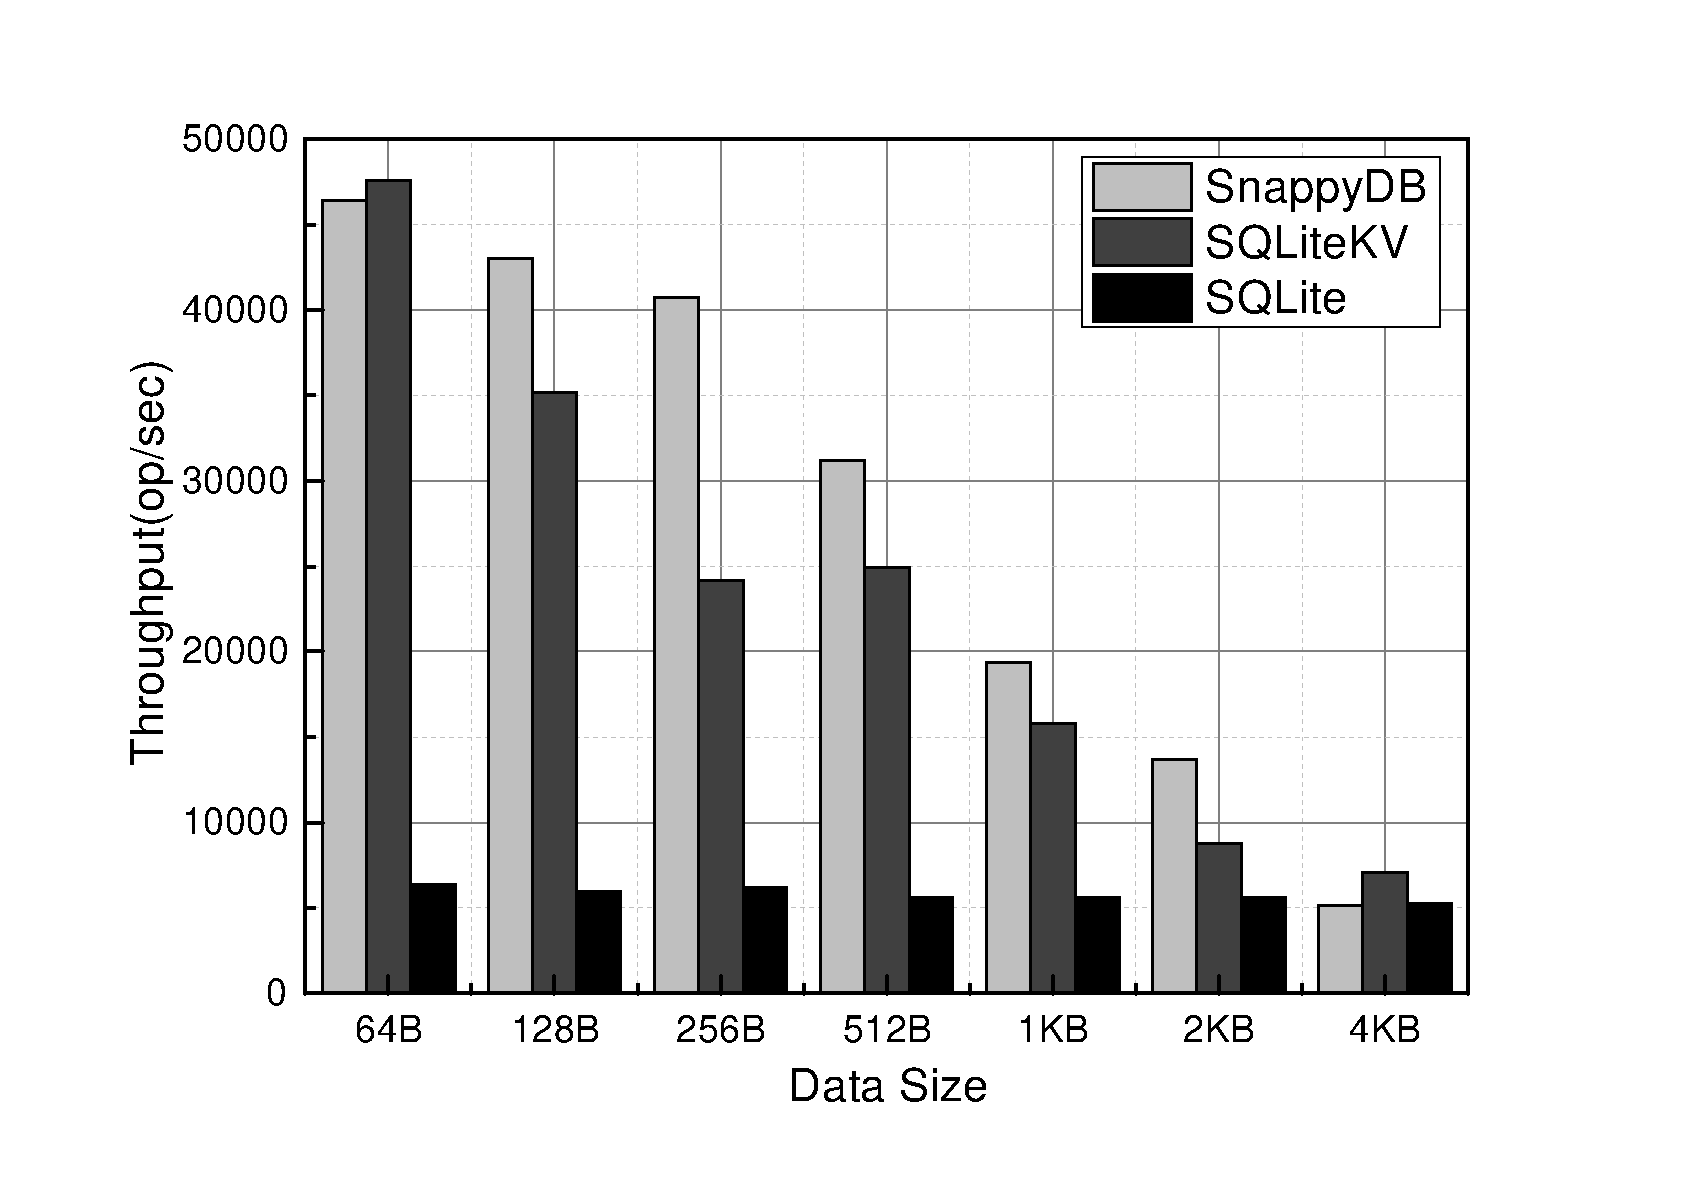
\includegraphics[width=0.9\textwidth, height=3.5cm]{Ext/workload4.pdf}
		\vspace*{-0.2cm}
		\caption{\small Throughput w. Read Latest Workload.}
		\label{fig:workload4}
	\end{minipage}
	
	\caption{\small Overall Performance}
	\label{fig:overallPerformance}
\end{figure*}
Figure \ref{fig:overallPerformance} shows the experimental results by running SnappyDB, SQLiteKV, and SQLite with the four workloads in ~\ref{table:workload}. For each workload, the key-value item sizes vary from 64 bytes to 4096 bytes. It can be observed that when the key-value item size is less than 2048 bytes, compared with SQLite, SQLiteKV significantly increases the throughput (operations per second). For example, the throughput with the 64-byte key-value items is improved by over 6.1 times. At the same time, with the same configuration (64-byte key-value), SQLite introduces from 18.2\% to 40.76\% throughput degradation against SnappyDB. As most data sets in SQLite with mobile applications are dominated with small requests (i.e. less than 100 bytes ~\cite{atikoglu2012workload}), we believe it is worthwhile for SQLiteKV to scarify this overhead while providing a SQLite interface.     

When the key-value sizes are over 2048 bytes, SQLiteKV, as well as SnappyDB, does not significantly outperform SQLite. The reason is that for LSM-tree-based databases, keys and values are written at least twice: the first time for the transactional log and the second time for storing data to storage devices. Thus, the per-operation performance of SQLiteKV is degraded by extra write operations. Regardless of this degradation, since most data sets in mobile applications only contain very few large requests, SQLiteKV can still significantly outperform SQLite in practice.    

To check the influence with the different insertion/query ratios, we use the case with 128-byte KV items as an example. For the Update Heavy workload, for SQLiteKV, the throughput is 20\% higher than that with the Read Heavy workload. The main reason is that in LSM-tree-based databases, for randomness-dominated workloads as these we use, write efficiency is better than read efficiency ~\cite{sears2012blsm}. For SQLiteKV, the similar trends can be observed from other workloads. 

In summary, SQLiteKV can significantly outperform SQLite by over 6 times on throughput for different workloads with various insertion/query ratios when the sizes of requests are small (no more than 128 bytes).  



\section{Performance with Different Sequential/Random Workloads}
In the second set of experiments, we investigate the impact of random and sequential accesses on SQLiteKV, SQLite and SnappyDB. Here, the key size is 16 bytes and the value size varies from 64 bytes to 4096 bytes. Next, we present the results related to insertions and queries, respectively.  

\subsubsection{Insertion Performance}
Figure ~\ref{fig:S-write} shows the results with random and sequential insertion operations, respectively, in which the key-value size varies from 64 bytes to 4096 bytes. For the sequential case, the key space is traversed in ascending order, while it is randomly traversed for the random case. 

It can be observed that for SQLitKV its insertion performance with sequential records is better than that with random records (the average improvement is 40\%). SnappyDB shows the simlar trend to SQLiteKV. On the contrary, for SQLite, there are no differences between the random and sequential cases, as its records are organized via B-Tree indexes.      

\begin{figure*}
	\centering
	\begin{subfigure}[b]{0.4\textwidth}
		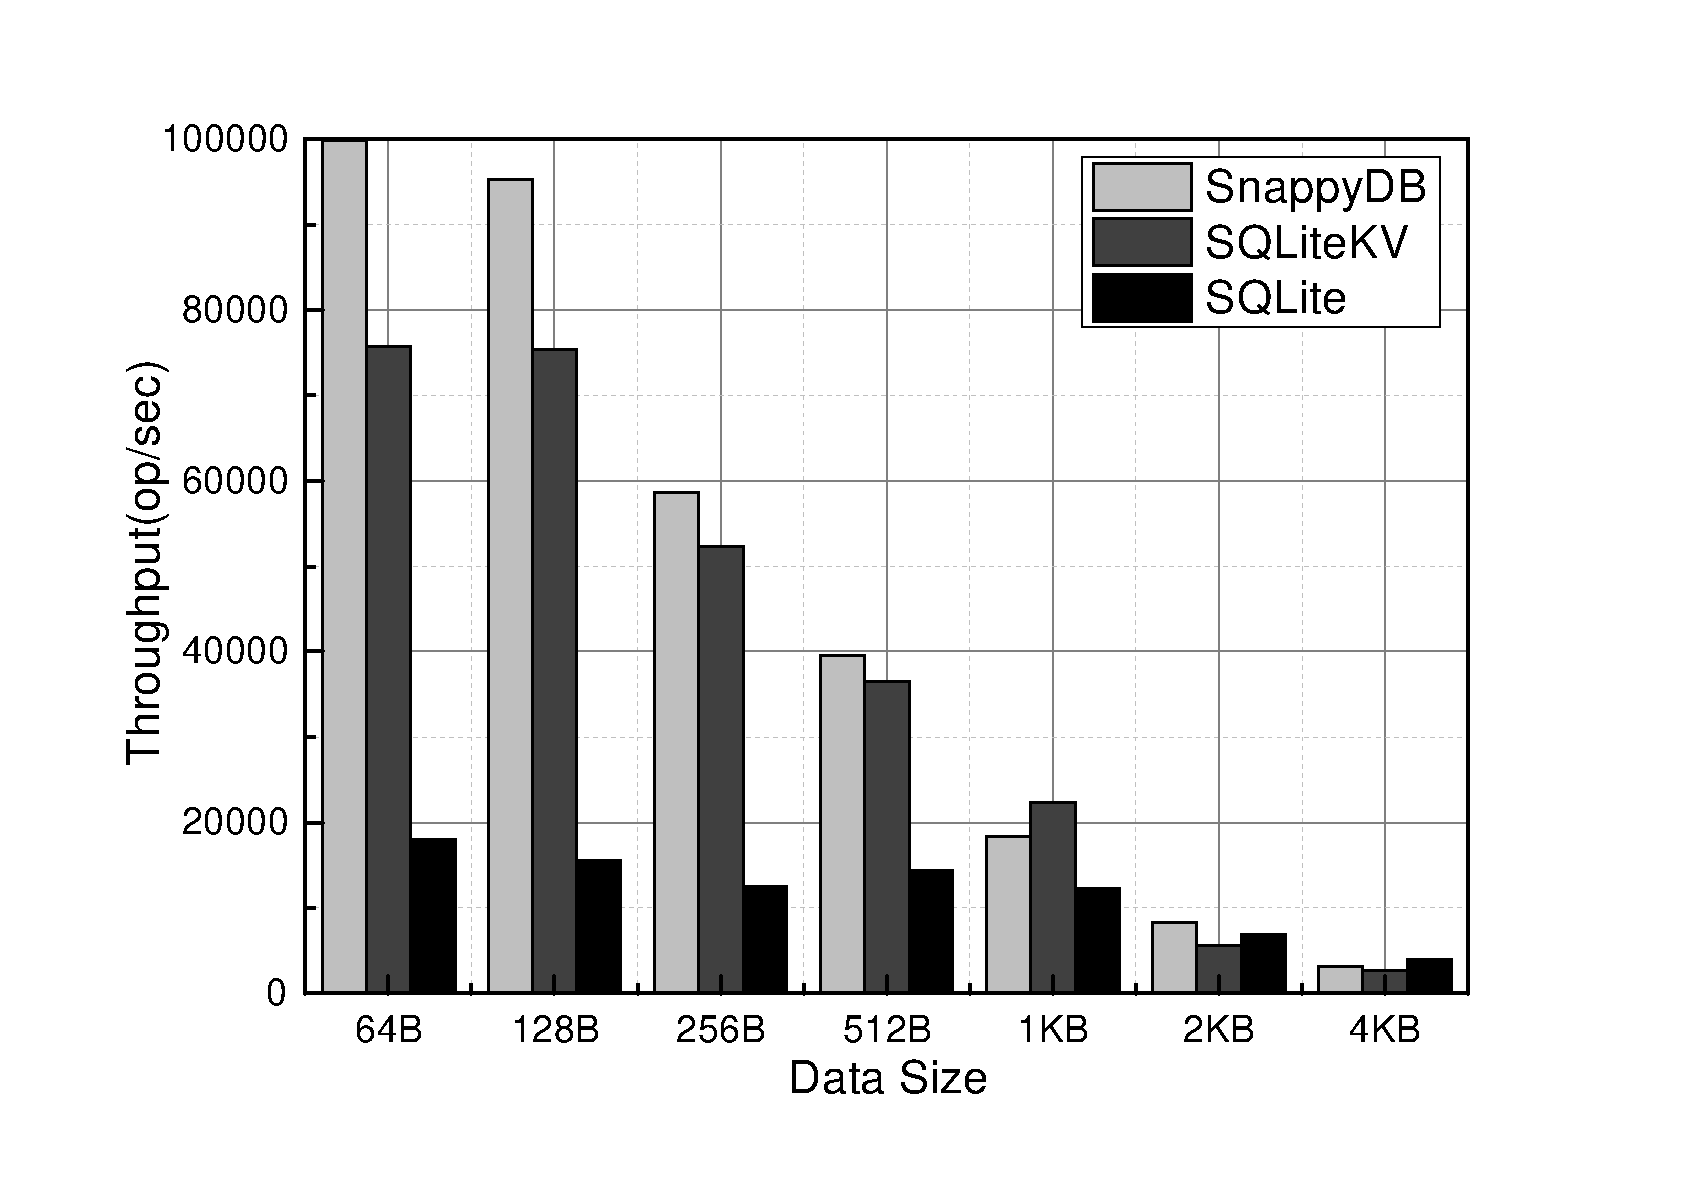
\includegraphics[width=0.9\textwidth, height=3.5cm]{Ext/R-Write.pdf}
		\caption{\small Random Insertions.}
		\label{fig:R-write}
	\end{subfigure}
	\hspace{0.7cm}
	\begin{subfigure}[b]{0.4\textwidth}
		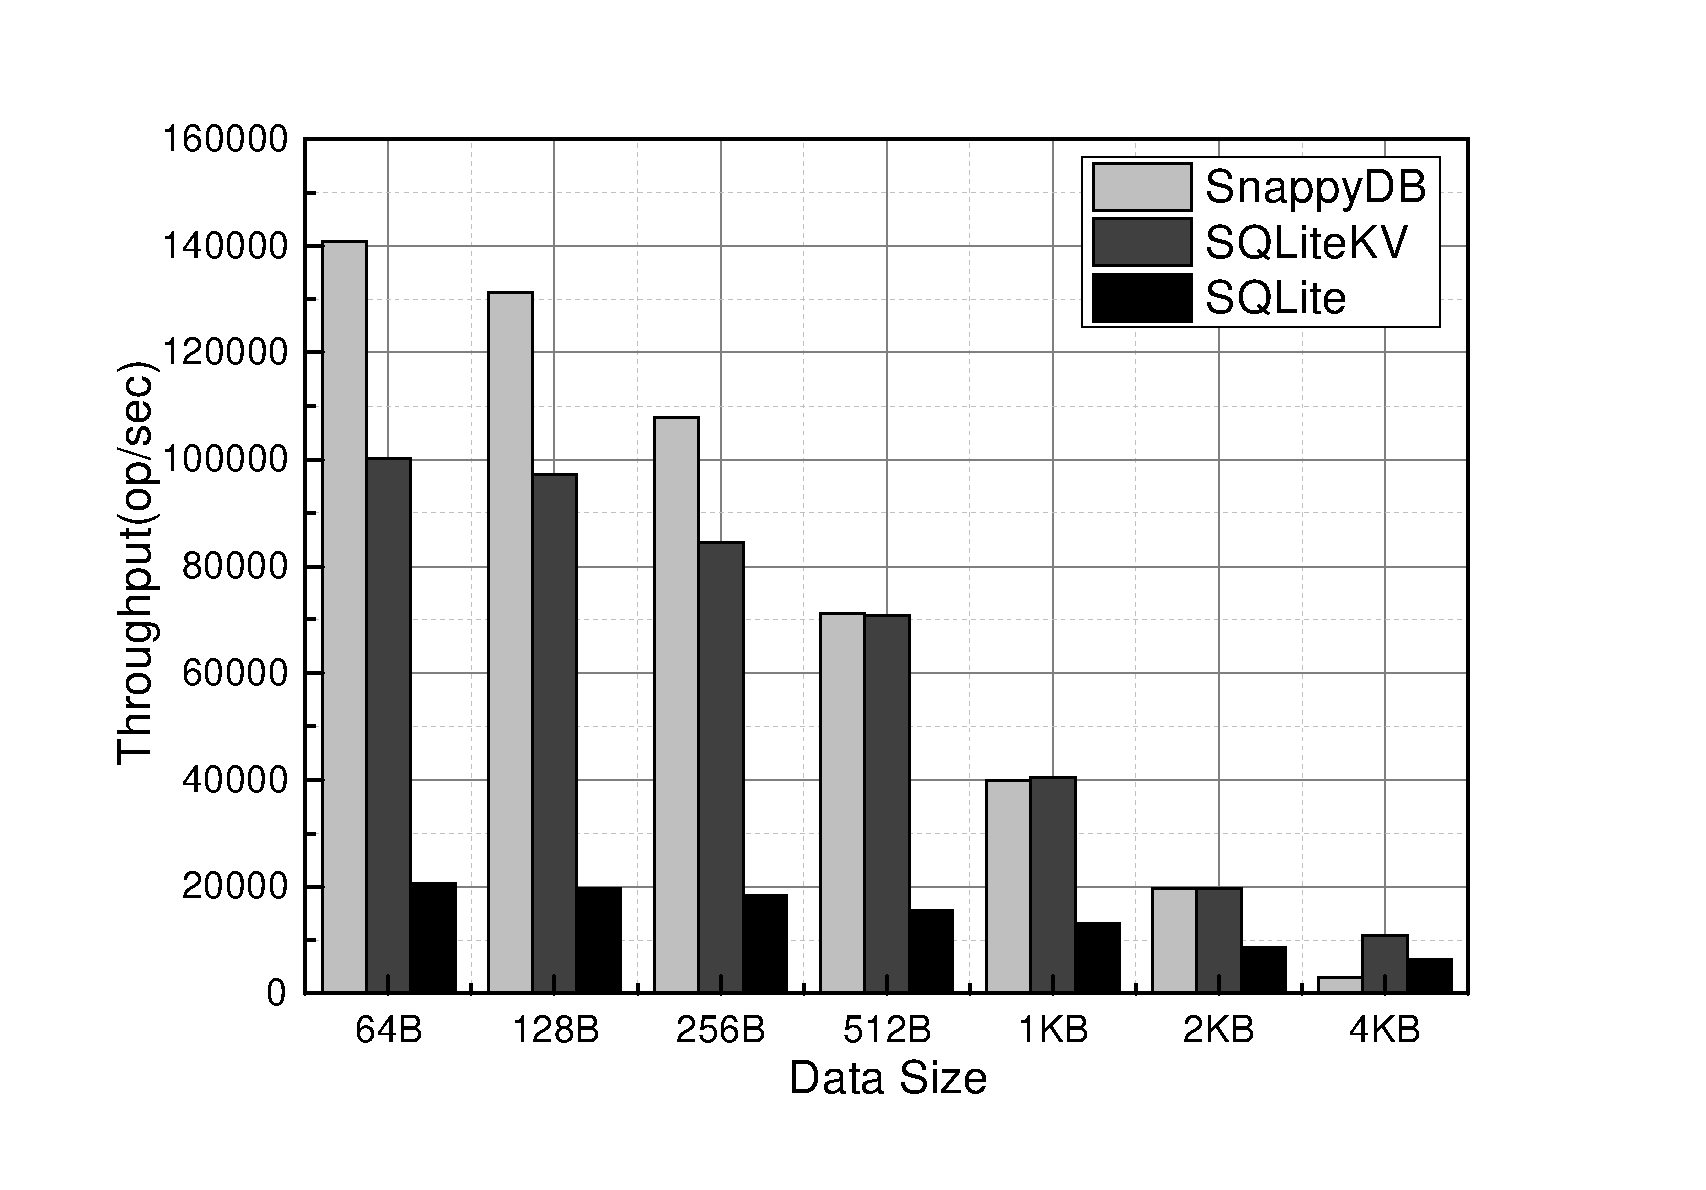
\includegraphics[width=0.9\textwidth, height=3.5cm]{Ext/S-Write.pdf}
		\caption{\small Sequential Insertions.}
		\label{fig:S-write}
	\end{subfigure}
	\caption{\small Insertion Throughput vs. KV size}
\end{figure*}

\begin{figure*}
	\centering
	\begin{subfigure}[b]{0.4\textwidth}
		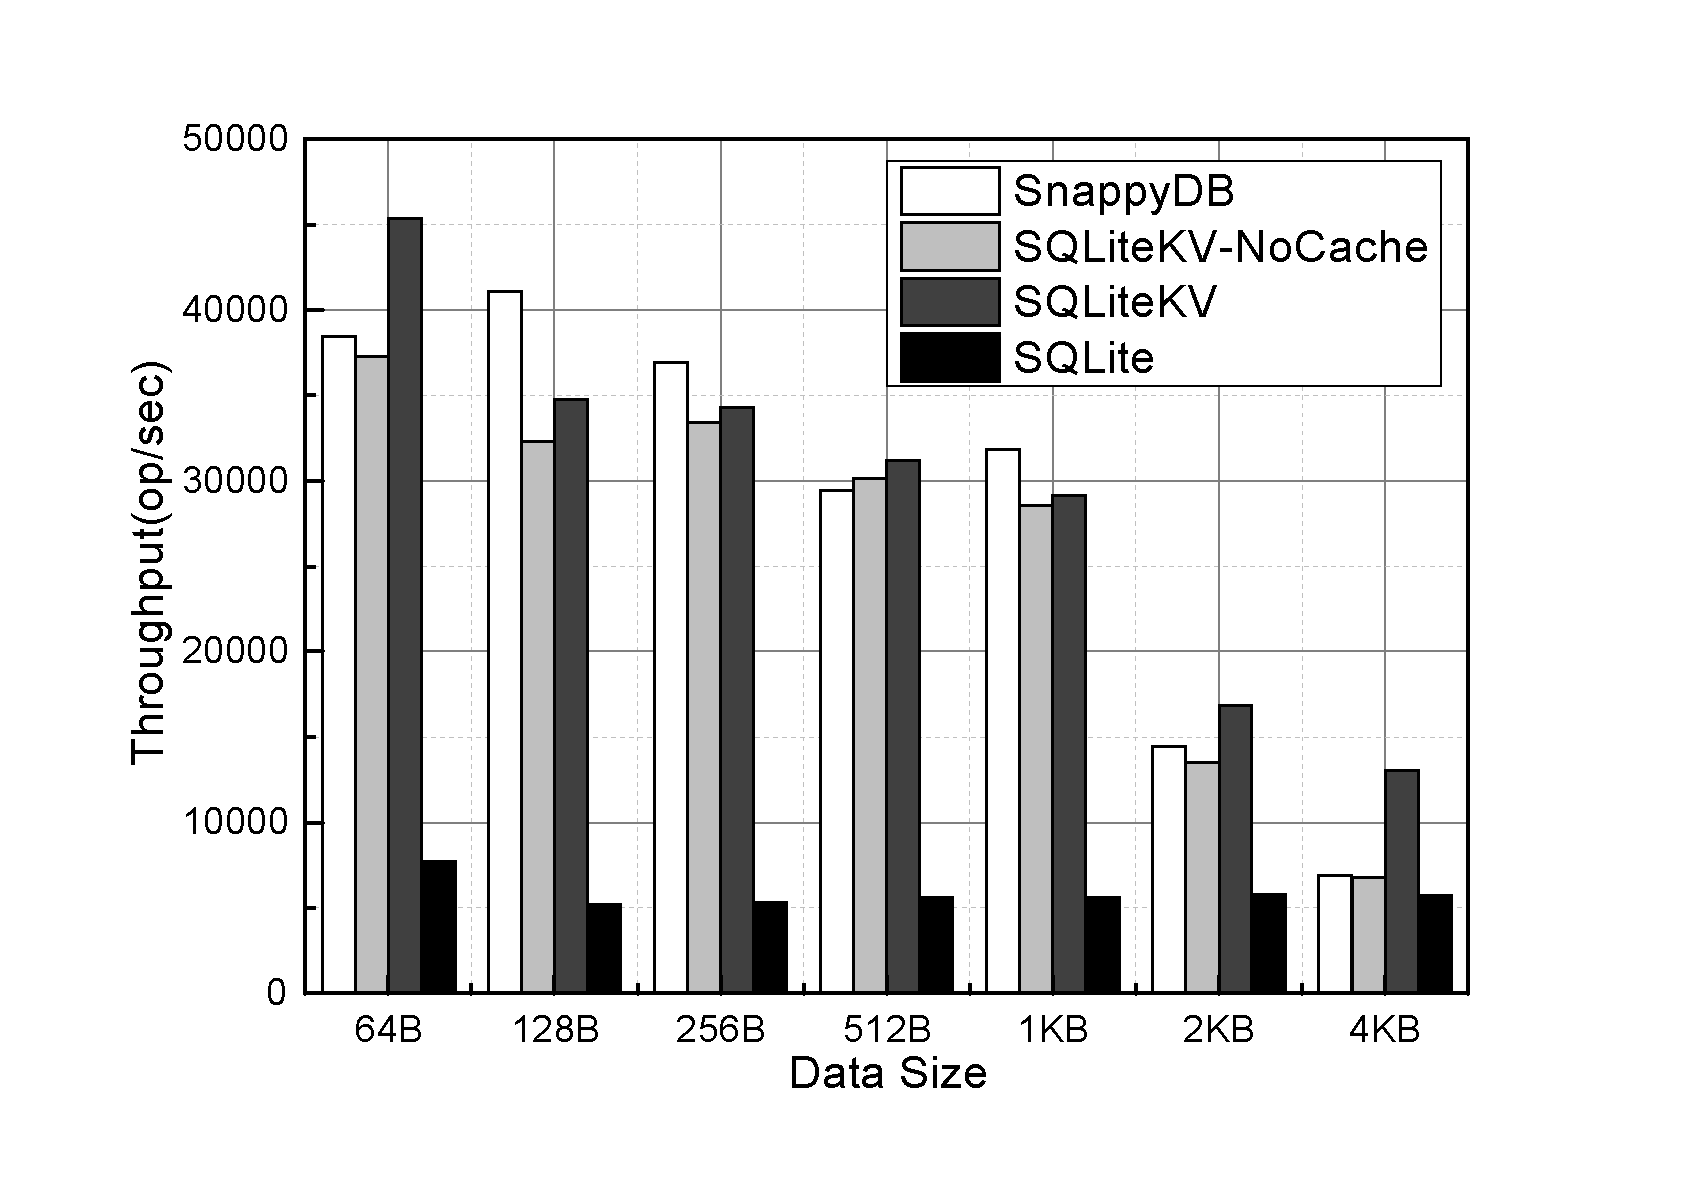
\includegraphics[width=0.9\textwidth, height=3.5cm]{pic/R-read.pdf}
		\caption{\small Random Queries.}
		\label{fig:R-read}
	\end{subfigure}
	\hspace{0.7cm}
	\begin{subfigure}[b]{0.4\textwidth}
		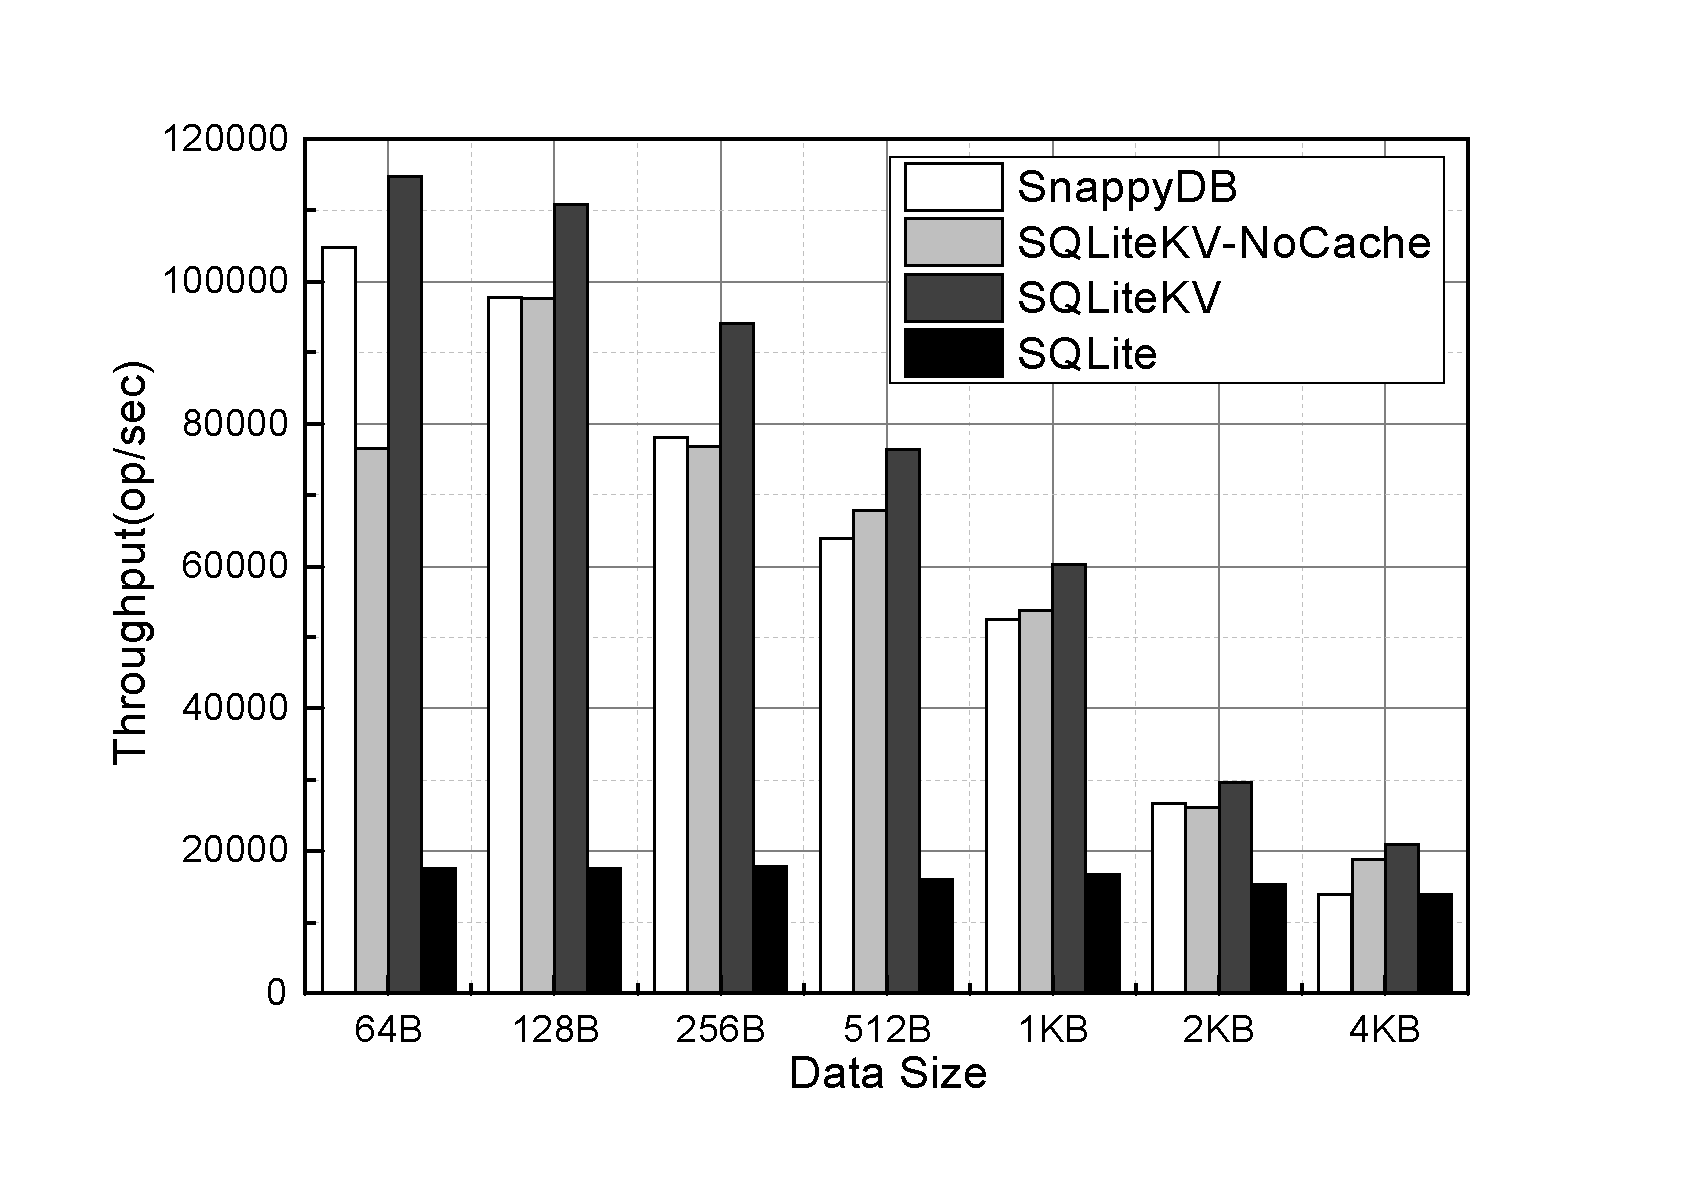
\includegraphics[width=0.9\textwidth, height=3.5cm]{pic/S-read.pdf}
		\caption{\small Sequential Queries.}
		\label{fig:S-read}
	\end{subfigure}
	
	\caption{\small Query Throughput vs. KV size}
	\label{fig:queryPerformance}
\end{figure*}
\subsubsection{Query Performance}
Similarly, Figure ~\ref{fig:S-read} shows the results with random and sequential query operations, respectively. The similar trends can be observed as with insertion operations. Specially, for SQLitKV, its query performance with sequential records is much better than that with random records (the average improvement is around 2 times). 

In Figure ~\ref{fig:S-read}, we also present the results for SQLiteKV without cache. Compared with SQLiteKV, it can observed that our slab-allocation caching mechanism can help improve 10 - 20 \% query performance. Furthermore, it can provide a noteworthy improvement, up to 2.x times, on large data sets.

 \chapter{Conclusion}
\label{chap:sumup}
In this paper, we proposed SQLiteKV that is a SQLite-like key-value database engine. SQLiteKV adopts the LSM-tree-based data structure but retains the SQLite operation interfaces. It consists of two parts, a front end that contains a light-weight SQLite-to-key-value compiler and a cache, and a back end that contains a LSM-tree-based key-value database engine. 
We have implemented and deployed our SQLiteKV on a Google Nexus 6P Android platform. The experimental results with various workloads show that SQLiteKV can significantly outperform SQLite. 
 
\startbibliography
 \begin{singlespace} % Bibliography must be single spaced
  \bibliography{References}   % Use the BibTeX file ``References.bib''.
 \end{singlespace}

% An external Abstract that can be printed at the end of the document, 
% for separate submission to Rackham. Comment it out when not needed. - jg
%\startextabstractpage
%{The Title of Your Dissertation}{Your Name}{Chair: Albert Einstein}
%SQLite has been deployed in millions of mobile devices from web to smartphone applications on various mobile operating systems. However, SQLite is not efficient with low transactions per second. In this paper, we for the first time propose a new SQLite-like database engine, called SQLiteKV, which adopts the LSM-tree-based data structure but retains the SQLite operation interfaces. With its SQLite interface, SQLiteKV can be utilized by existing applications without any modification, while providing high performance with its LSM-tree-based data structure.

In SQLiteKV, we develop a light-weight SQLite to key-value compiler to solve the semantic mismatch, so SQL statements can be efficiently translated into KV operations. We also design a novel coordination caching mechanism with memory defragmentation so query results can be effectively cached inside SQLiteKV by alleviating the discrepancy of data management between front-end SQLite statements and back-end key-value data organization. We have implemented and deployed SQLiteKV on a Google Nexus 6P smartphone. Experiments results show that SQLiteKV outperforms SQLite up to 6 times.
%\label{ExtAbstract}

\end{document}